%
% TEBNF Project Report
%
% Jason Young
%
% Based on the USU thesis and dissertation template (Rev. 31) last
% last modified Wed Oct 10 12:16:55 2007 by Scott Budge <scott@goga.ece.usu.edu>
%

\documentclass[cs,msreport]{usuthesis}

% Packages
\usepackage{amssymb}           % add ams symbols stuff
\usepackage{caption} 
\usepackage{graphicx}          % add graphics
\usepackage{subfigure}
\usepackage{xcolor,colortbl}   % table cell coloring

\captionsetup[table]{skip=10pt} % adds spacing between tables and captions

% Author and Title Information
\author{Jason G. Young}
\title{Code Generation: An Introduction to Typed EBNF}

% The Committee
\majorprof{Dr. Vicki H. Allan}
\firstreader{Dr. Kenneth Sundberg}
\secondreader{Dr. Curtis Dyreson}

% Graduate Dean
%\graddean{Dr. Mark R. McLellen} 
%\deantitlea{Vice President for Research and}
%\deantitleb{Dean of Graduate Studies}

% Degree Information
\degree{Master of Science}
\month{May}
\year{2015}

\begin{document}
    % Frontmatter
    \preliminaries         % set frontmatter style
    
    \maketitle
    \makecopyright         % optional    

    \begin{abstract}
% A space is needed before the text starts so that the first paragraph
% is indented properly.

Errors and inconsistencies between code components can be very costly in a software project.  Efforts to reduce these costs can include the use of tools that limit human interaction with code by generating it from a description.  Most of these tools only generate one of the many components found in a typical application, reducing human-introduced errors within code.   This paper introduces two new works: (1) an input specification called Typed EBNF (TEBNF), and (2) a prototype tool that demonstrates how TEBNF can be used to generate code.  The tool generates code for a console application as described by a TEBNF grammar.  An application built from the generated code will be able to receive input data, parse it, process it, and output it as needed.

\end{abstract}

    %%
% This is an example of an dedication page.  This is optional,
% and can contain anything you want to say.
%
%  (last_modified) Wed Oct 10 12:21:36 2007 by Scott Budge <scott@goga.ece.usu.edu>
%
%  Info: $Id: dedication.tex 31 2007-10-11 14:52:59Z scott $   USU
%  Revision: $Rev: 31 $
% $LastChangedDate: 2007-10-11 08:52:59 -0600 (Thu, 11 Oct 2007) $
% $LastChangedBy: scott $
%

\begin{dedication}
\begin{center} 
To all the little people....
\end{center}
% 
% If you intend to have a dedication longer than one line, do not put
% it in a centering environment.  It will look better.
\end{dedication}
  % optional 
    %%
% This is an example of an acknowledgements page.  This is optional,
% and can contain anything you want to say.
%
%
%  (last_modified) Wed Oct 10 15:00:26 2007 by Scott Budge <scott@goga.ece.usu.edu>
%
%  Info: $Id: acknowl.tex 31 2007-10-11 14:52:59Z scott $   USU
%  Revision: $Rev: 31 $
% $LastChangedDate: 2007-10-11 08:52:59 -0600 (Thu, 11 Oct 2007) $
% $LastChangedBy: scott $
%

\begin{acknowledgments} 
I am so happy that my advisor helped me.....
\\
\begin{flushright} 
John Q. Engineer 
\end{flushright}
\end{acknowledgments}

     % optional
    
    \tableofcontents 
    \listoftables 
    \lstlistoflistings
    \listoffigures

    \body
    \chapter{Introduction}
Various defects in software can result from multiple developers working on the same code within a project \cite{livshits_01}.  Some errors introduced by the coding activities of developers may consist of behavioral differences within and between components and their interfaces \cite{leveson_01,smidts_01,nakajo_01}.  Other errors stem from inadequate comprehension of project code, supported by the fact that developers spend 50\% to 80\% of their time understanding it \cite{sinha_01}.  Furthermore, these kinds of misunderstandings can lead to bug fixes that inject more faults into code \cite{smidts_01}.

\indent
Comprehensive requirements analysis, design, and other good software development practices can prevent many post-delivery software problems \cite{boehm_01}, but cannot completely eliminate the possibility of human error.  Even well designed projects can get mired in code implementation details that hinder or prevent developers from delivering on time and within budget.

\section{Code Generation}
Code generation tools can improve the software development process by generating well-organized code reducing implementation errors and inconsistencies \cite{boysen_01}.  Code generation has been shown to improve the productivity of developers, guarantee correctness of syntax, and decrease errors \cite{groher_01}.  A compiler is a type of code generation tool that generates binary executables from code written in higher-level programming languages like C and C++.   Some tools generate higher-level code instead of binary given a set of rules known as a grammar.  This high-level generated code is then fed to a compiler to create a binary executable.

\indent
Most high-level code generation tools are specialized and only generate one part of an application'’s overall implementation.  Popular targets for specialized code generation are lexical analyzers and parsers.  One of the earliest code generation tools is the compiler-compiler (parser generator), a term first presented in the early 1960’s \cite{brooker_01}.

\section{TEBNF Input Specification and Code Generation Tool}
This report will present a new input specification based on Extended Backus-Naur Form (EBNF) called Typed-EBNF (TEBNF) (see appendix~\ref{appendix:TEBNF}), and a new prototype code generation tool that uses TEBNF as its input specification.  The tool will validate key features of TEBNF:
\begin{itemize}
  \item TEBNF grammars can describe input patterns that include a mixture of strings, numbers, and/or raw groupings of bytes.
  \item TEBNF integrates grammar rules with states and actions.
  \item TEBNF can specify different methods of receiving input and sending output.
  \item TEBNF can declare how raw input data should be unmarshaled into well-known types of specific sizes (in bytes).
  \item TEBNF can declare how well-known types should be marshaled back into their original format.
  \item TEBNF provides typed and non-typed EBNF terminals.
  \item TEBNF supports arithmetic and non-arithmetic operations inside grammar rules.
  \item TEBNF grammars match specific pieces of a given input to well-known types of varied sizes (in bits or bytes).
  \item TEBNF supports the use of variables.
  \item TEBNF is Turing complete (see appendix~\ref{appendix:TEBNFTuringCompletenessProof}).
\end{itemize}

\indent
The prototype code generation tool will demonstrate that it can generate a console application that can (1) parse data from different kinds of inputs, (2) process data to produce specific output(s), (3) direct output(s) to a network destination (UDP/IP), file, or console-based user-interface, (4) support custom network protocol handling and interaction (UDP/IP), and (5) provide a console-based user interface for the application.
 % Introduction
    \chapter{Background and Related Works}
The purpose of code generation tools is to help developers improve their productivity, ensure correctness of code syntax, and lessen the number of errors in software \cite{groher_01}.  The input specifications of these tools introduce additional levels of indirection to solve these problems \cite{spinellis_01}.  A range of tools have been created to generate code that can be complex and tedious to write by hand:
\begin{itemize}
  \item Scanners
  \item Parsers
  \item Interpreters
  \item Compilers
  \item Graphical user interfaces
\end{itemize}

\section{Traditional Scanner and Parser Code Generation}
The Yacc (“Yet Another Compiler Compiler”) \cite{johnson_01} first introduced in 1975 is a popular tool that generates LALR parsers given (1) a context-free grammar to describe input, (2) an action (code snippets) to run for each token grouping that matches a grammar rule, and (3) code to provide input tokens to the parser.  This input specification is a hybrid between a declarative domain-specific language (i.e. a grammar) and an imperative programming language like C \cite{demetrescu_01,lloyd_01,gifford_01}.  Nevertheless, Yacc lacks the ability to read an input stream and convert it into tokens for parsing.

\indent
Lexical analyzer generators such as Lex and Flex must be used in conjunction with Yacc to accomplish this separate task of lexical analyzer generation \cite{johnson_01,lesk_01}.  The practice of using separate tools to generate a lexical analyzer and parser mean that input formats for each tool must be learned and used correctly to achieve the desired result.

\begin{figure}[htbp]
\centering
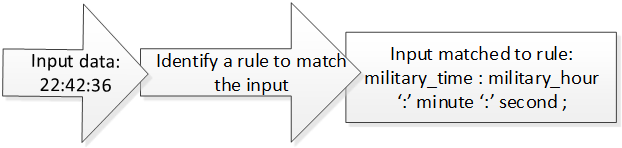
\includegraphics[width=0.9\textwidth]{figures/YaccGrammarRule.png}
\caption{Example Yacc grammar rule matched to input.}
\label{fig:YaccGrammarRule}
\end{figure}

\indent
Figure~\ref{fig:YaccGrammarRule} shows an example Yacc grammar rule matched to input formatted as military time.  In this example, military\_hour, minute, and second (all defined somewhere else in the grammar) describe specific parts of input data as military\_time.  When tokens match this rule, a code action is executed \cite{johnson_01,niemann_01}.

\indent
Similar to Yacc is Bison \cite{aycock_01,demaille_01}, a Yacc-compatible parser generator that accepts any properly written Yacc grammar.  Like Yacc, Bison-generated parsers read a sequence of tokens from a scanner generated by a lexical analyzer generator like Lex or flex.

\indent
To illustrate the steps of traditional parser generation using Lex and Yacc (figure ~\ref{fig:YaccGrammarRule}) \cite{johnson_01,lesk_01,niemann_01}, a file is provided by the developer containing a set of patterns that define how to separate strings found in source data.  This file is read by Lex, which uses these patterns to generate the C source code of a lexical analyzer.  This newly generated lexical analyzer uses the patterns to identify specific strings in the input and split them into tokens to simplify processing.

\begin{figure}[htbp]
\centering
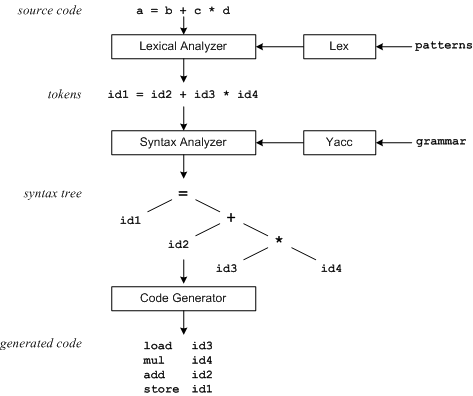
\includegraphics[width=0.9\textwidth]{figures/LexAndYaccCompileSequence.png}
\caption[Lex and Yacc Compilation Sequence]{Lex and Yacc Compilation Sequence \cite{niemann_01}.}
\label{fig:LexAndYaccCompileSequence}
\end{figure}

\indent
A file containing grammar rules is provided by the developer to Yacc, which uses those rules to generate C source code for a syntax analyzer (i.e. parser).  The syntax analyzer uses this grammar to transform the tokens output by the lexical analyzer into a syntax tree.  The structure of this syntax tree implies the precedence and associativity of operators found within the tokens.  The syntax tree is then traversed in depth-first order to generate the desired source code (figure ~\ref{fig:LexAndYaccCompileSequence}) \cite{niemann_01}.

\indent
A predicated-LL(k) parser called ANTLR \cite{parr_01} was introduced by Parr and Quong in 1995.  The ANTLR parser generator was advertised to be easier to use than generators like YACC or BISON.  An LL(k) parser is a top-down parser that parses from left to right, utilizing a look-ahead of k tokens.  All parsing decisions are made solely from the next k tokens, which means that it does no backtracking.

\indent
The HYACC (Hawaii Yacc) parser generator first released in 2008 supports complete LR(0), LALR(1), LR(1), and partial LR(k) \cite{chen_01,chen_02}.  HYACC is compatible with Yacc and Bison input grammars and works with Lex.  The HYACC parser generator is notable because it can resolve reduce/reduce conflicts through its implementation of the LR(1) parser generation algorithm \cite{chen_01}.  Reduce/reduce conflicts occur when two or more rules in an input grammar apply to the same input sequence \cite{free_01}.  These conflicts are typically the result of a serious problem with an input grammar \cite{free_01}.

\indent
The traditional code generation process using a lexical analyzer generator in conjunction with a parser generator and actions code is shown in figure~\ref{fig:TraditionalCodeGenProcess}.  This process illustrates the pattern used by many parser generation tools.

\begin{figure}[h!]
\centering
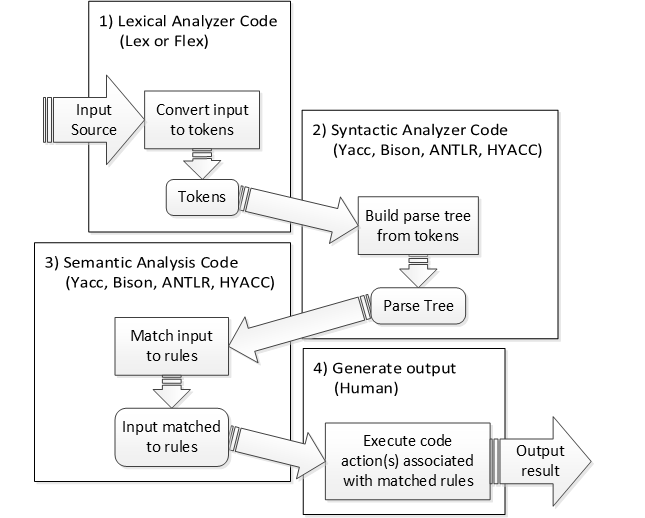
\includegraphics[width=0.9\textwidth]{figures/TraditionalCodeGenProcess.png}
\caption{Traditional code generation process.}
\label{fig:TraditionalCodeGenProcess}
\end{figure}

\indent
All of these parser generators provide an effective means to reduce human interaction with code.  They have the added benefit of generating logical and syntactically correct code as long as the grammar is correct.  On the other hand, the input grammars used by these parser generators cannot be used for lexical analysis of the parser input.  Moreover, code actions that generate output are not provided as part of the input grammar.  These actions must be manually written and inserted into the code generated by the parser generator.

\section{Model-Based Parser Code Generation}

\indent
Model-based parser generators provide an alternative to traditional parser generators using a model-based language specification.  This kind of specification is explained by \cite{quesada_01} and \cite{quesada_02} as starting with an abstract syntax model (ASM) embodying the main concepts of a given language.  One or more concrete syntax models (CSMs) are created from this ASM.  Each CSM defines specific details about the language being modelled.  Elements within the ASM can then be converted into their concrete representation using a mapping of the ASM to its CSM(s).  This mapping is created by annotating the ASM with pertinent constraint metadata.  With this mapping in place, any changes to the ASM by the user will cause the language processor to automatically update to reflect those changes.  Figure~\ref{fig:ModelBasedCodeGenProcess} illustrates the model-based parser code generation process.

\begin{figure}[h!]
\centering
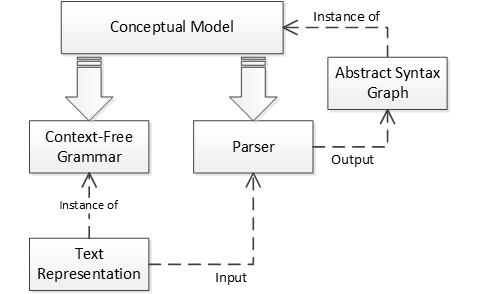
\includegraphics[width=0.9\textwidth]{figures/ModelBasedCodeGenProcess.png}
\caption[Model-based code generation process.]{Model-based code generation process, based on a figure from \cite{quesada_02}.}
\label{fig:ModelBasedCodeGenProcess}
\end{figure}

\indent
Since grammar specifications are not needed by model-based parser generators they can offer several advantages over traditional parser generators \cite{quesada_02}:
\begin{itemize}
  \item An easier language design process.  Language design is decoupled from language processing because the language grammar is automatically generated.
  \item Non-tree structures can be modeled.  This is different from traditional parser generators that force users to model a tree structure.
  \item Some semantic checks like reference resolution can be automated.
  \item Handles references between language elements, as opposed to the traditional way of resolving references manually using a symbol table.
\end{itemize}

\indent
Model-based parser generators can behave in one of two ways based on the ASM used \cite{quesada_02}: (1) as a traditional parser generator when an ASM representing a tree structure is used, or (2) as a model-based parser generator when an ASM representing a non-tree structure is used.   The second possibility causes a model-based parser generator to begin the reference resolution process, resulting in an abstract syntax graph.

\indent
ModelCC is a model-based parser generator that accepts an annotated conceptual model as its input rather than a context-free grammar \cite{quesada_01}.  ModelCC uses this annotated model to generate a parser written in Java that automatically instantiates the language conceptual model \cite{quesada_01, modelcc_01}.

\indent
The process of generating a parser using ModelCC as explained by \cite{quesada_02} begins with an ASM that is defined by classes representing language elements and the relationships between them.  Metadata annotations are added to these language elements and their corresponding relationships to produce an ASM to CSM mapping.  Reference resolution is performed to match referenced objects to their equivalent object instantiations.  A parser is then generated that automatically instantiates the conceptual model.

\indent
ModelCC effectively decreases human interaction with code by generating grammar code and lexical analysis code from an input model specification.  On the other hand, it is similar to other parser generators because it does not implicitly support specific input/output methods such as UDP/IP, etc.

 % Background and Related Works
    \chapter{Design}
The TEBNF language makes it possible to convert a software design expressed as a state machine and convert it into a specification that can be provided to the TEBNF code generation tool.  The TEBNF code generation tool generates C++ 11 code from TEBNF grammars that can be built by a C++ compiler into a functioning console application.  This chapter discusses the TEBNF language, design decisions, the TEBNF code generation tool, the architecture of the tool, and the code generation process.

\section{The TEBNF Language}
The TEBNF specification is composed of language constructs called elements.  A TEBNF grammar is the combination of these elements and their contents to define an application.   The primary function of each element type is to convey one specific functionality.  One advantage of this approach is scalability.  The complexity of each element is reduced because each element does one thing only.  This follows the established design paradigm of making something do only one thing but do it well.  There are five kinds of elements in the TEBNF specification:
\begin{itemize}
  \item Input methods: a method of receiving data as input.
  \item Output methods: a method of outputting data.
  \item Grammar sections: parses input data. 
  \item Actions: action code to execute using data from other elements.
  \item State transition tables: defines execution path.
\end{itemize}

\indent
Within each element are separate constructs known as subelements.  Different kinds of subelements exist for each element type, and are enumerated in detail in appendix~\ref{appendix:TEBNF}.  The glue that brings these elements together to describe an application is two-fold: 1) static variables that can be defined within grammar elements and used by other elements to get and store information, and 2) state transition table elements that use all of the other elements in a grammar to express the order of task execution.

\subsection{Design Decision: Singleton Paradigm}
One of the primary goals of TEBNF is to reduce the difficulty of translating high-level designs into grammars.  Keeping TEBNF simple means that developers are spending more time designing how an application will be used rather than worrying about many of the details associated with translating their design into code.   Elements have been designed to behave as singletons in TEBNF, as well as the code generated from them.

\indent
Multiple reasons and advantages exist for treating TEBNF elements and the C++ classes generated from them as singletons:
\begin{itemize}
  \item Lazy instantiation.  Singleton C++ classes make it possible to avoid allocating memory for element class objects until they are actually used in the generated code.  This is different from static initialization that allocates memory to a variable at the time of declaration.
  \item Thread synchronization.   Singletons can yield the best results in situations where multiple threads try to access the same resource.  This applies to code generated from a TEBNF grammar because it is possible for multiple state table threads to need access to the same subelement or static variable class members at the same time.
  \item Instance control.  A singleton prevents other objects from instantiating their own copies of the singleton object, ensuring that all objects access the same instance.  This simplifies the design process in TEBNF because grammar writers know exactly what they are accessing in their grammar.
  \item Flexibility.  Generated singleton element classes control the instantiation process.  This control over the instantiation process gives them the flexibility to change the process.  Since TEBNF purposely abstracts these details from grammar writers, it is advantageous for each element class to control the way it is instantiated based on how it is used/interacts in the generated application code.
\end{itemize}

\subsection{Design Decision: Adapting TEBNF}
Some complexities in the TEBNF language were exposed as the code generation tool was written.  When encountered, adaptations to TEBNF were made to better represent their nature and interaction of these complexities within the language.  Design decisions made with respect to TEBNF elements are discussed in~\ref{ssec:IoElements} and~\ref{ssec:ActionsElements}.

\subsection{Design Decision: Input and Output Elements} \label{ssec:IoElements}
Console applications typically get string or numerical input from users by displaying questions and waiting for the user to type an answer.  Attempting to determine the type of input information in generated code could lead to incorrect interpretations of the input type at run time.  One technique that was considered to avoid this problem is to directly tie grammar subelements or static variables to input subelements.  This method proved to be unwieldy because grammar elements change during the natural process of writing a TEBNF grammar.  Simply changing the name of a grammar subelement would require that name to be changed in every input subelement tied to it.  This problem could be compounded as other input elements are created that contain subelements tied to the same grammar subelements or static variables.   To resolve this problem, console input subelements tie each question string to a type (appendix~\ref{appendix:TEBNF}).  The responsibility of knowing the expected input type falls to the grammar writer rather than a risky prediction.

\indent
Usage of console output elements in TEBNF was found to be simpler than console input.  This is due to the fact that generated console output code performs a simple passing of output data to a C++ std::cout statement.   Because std::cout easily handles outputting of numerical and string data, there is no need for special handling in TEBNF.

\indent
Support for sending and receiving data over UDP is achieved in TEBNF using UDP elements.  The TEBNF language uses UDP I/O elements to abstract most of the details involved with setting up and using UDP sockets.  Generated UDP I/O element classes prompt users for an IP address and port number before initiating UDP communication.  It became apparent that a way was needed to indicate that a UDP output element should send data on the same socket instance used by an existing UDP input element to receive data.  The "“AS"” keyword expresses this relationship between two I/O elements of the same type.  The “"AS"” relationship defines an element that shares all of the same characteristics as another I/O element of the same type.  Because TEBNF elements and their respective C++ element classes are singletons, all that is needed to represent this case in generated C++ code is a type definition of the I/O element in question (typedef).  This reduces the number of C++ classes generated.

\subsection{Design Decision: Actions Elements} \label{ssec:ActionsElements}
Actions elements in TEBNF share two similarities to C++ functions. The first similarity is the ability to have one or more parameters, allowing arguments to be passed inside state transition table elements.  Second, actions elements can contain multiple instructions.  Actions elements also allow grammar writers to access subelements and/or static variables found in any grammar element.  The syntax for accessing subelements defined inside other grammar elements can be found in appendix~\ref{appendix:TEBNF}.

\indent
Unlike C++ functions, actions elements cannot return values.  TEBNF purposely abstracts this kind of complexity from grammar writers.  This kind of functionality was intended to be expressed in state transition table elements.  In TEBNF, a “return value” is expressed in a state transition table when a state'’s input or condition criteria is met, resulting in data being routed (returned) to an output and/or optionally transitioning to a different state.  This supports their intended usage as the action(s) component of one or more states in a state machine.  A side effect of actions elements not returning values is that they cannot be used as the input or condition of a state within a state transition table element.  This is due to the fact that the resulting type of a state’s input or condition must be a Boolean.  This also illustrates one of the ways that TEBNF abstracts complexity through state machine design.

\indent
Actions elements are essentially C++ code blocks that allow direct reference to TEBNF subelements and static variables.  This means they have loose parsing requirements compared to other TEBNF elements so that the chosen C++ compiler can catch complex errors in actions element code.

\section{The TEBNF Code Generation Tool}
This report presents a prototype code generation tool that generates the lexical analysis, parsing, and actions code of a basic console application using a single TEBNF grammar as input.  Generated applications accept user input where necessary and can provide meaningful status.  The tool outputs a set of classes that:
\begin{enumerate}
  \item Accept input data through console, file, or UDP/IP.
  \item Provide a set of functions that unmarshal raw data into human-readable types such as numbers and strings, and can marshal it back into its original form.
  \item Use these unmarshal functions to match input data to pattern(s) specified in the grammar and convert them to human-readable values.
  \item Run one or more state machines with each on its own thread to receive data through input methods described in the grammar.  As input data arrives, the state machine finds matches to grammar patterns and executes actions that produce the desired output.
  \item Provide a console-based user interface that prompts for input as needed and provides status.
\end{enumerate}

\indent
The architecture of the TEBNF code generation tool consists of four stages, shown in figure~\ref{fig:TEBNFCodeGenToolArchitecture}.  The TEBNF code generation tool is a console application that accepts three arguments in order:
\begin{enumerate}
  \item Path of the file containing a TEBNF grammar.
  \item Path of directory where the tool will write generated code.
  \item The name to give to the generated application.
\end{enumerate}

\begin{figure}[h!]
\centering
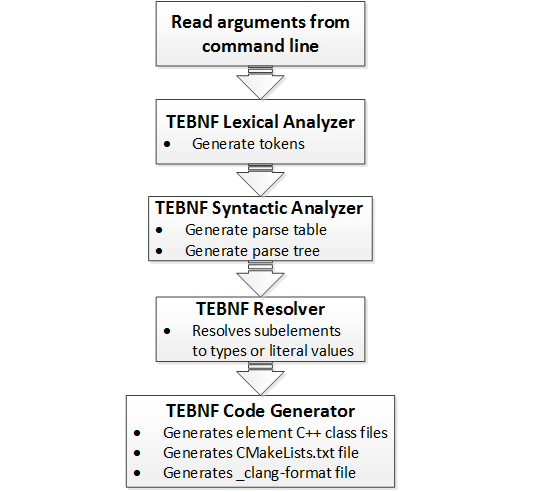
\includegraphics[width=0.9\textwidth]{figures/TEBNFCodeGenToolArchitecture.png}
\caption{Architecture of the TEBNF prototype code generation tool.}
\label{fig:TEBNFCodeGenToolArchitecture}
\end{figure}

\indent
Upon receiving these arguments, the tool reads the grammar file at the location provided to the tool.  The grammar is lexically analyzed by the TEBNF scanner to produce a list of tokens, with some metadata attached to some tokens as needed.

\indent
The TEBNF parser syntactically analyzes these tokens using a recursive descent algorithm to verify correctness of format.  A pointer to each element discovered by the parser is then added to a table for quick look up and inserted into a parse tree.  Subelements discovered during this parsing stage are added to their parent elements and subelements as they are found in the parse table and parse tree.

\indent
After all of the elements and subelements have been added to the parse table and parse tree, the TEBNF resolver traverses the subelements in the parse tree and their descendants to their furthest extent (leaves).  This ensures that all subelements resolve to a terminal type or literal value.

\indent
After all elements and their subelements have been resolved, the TEBNF code generator iterates through each element in order of declaration in the input grammar, and generates a C++ class or other appropriate C++ code.  The name of each C++ source file corresponds to the element it was generated from.  A CMakeLists.txt file is generated with these C++ source files so that CMake can be used to generate Microsoft Visual Studio 2013 solution and project files.  For convenience, a \_clang-format file is generated so that any clang-formatting (optional) follows the intended format.

\section{Lexical Analysis and Parsing Code Generation}
The TEBNF code generation tool generates a class for each input/output (I/O) element (method) defined in a TEBNF grammar (see appendix~\ref{appendix:TEBNF}).  These I/O classes perform no lexical analysis.  They only receive input and/or send output.  Supported I/O methods are as follows:
\begin{itemize}
  \item Console
  \item File
  \item UDP/IP
\end{itemize}

\indent
These I/O methods are a powerful feature of TEBNF and the TEBNF code generation tool because the tool automatically integrates the code to do I/O using these methods.  The complexities of their usage are abstracted by the tool, which is one of the key advantages of TEBNF and the TEBNF code generation tool.  Contrast this to the most common code generation tools, which do not provide this built-in I/O capability.

\indent
Lexical analysis and parsing is performed by the generated code in one step rather than separate steps.  This is possible because of the way patterns are described in TEBNF grammar elements (see appendix~\ref{appendix:TEBNF}).  A typical grammar element pattern is composed of groupings of bytes broken into sub-groupings of bytes.  These sub-groupings can be translated into specific types (e.g. numbers, and strings) and literal values.  The size in bits or bytes is defined in the grammar element based on its type.

\indent
Matching user-defined TEBNF grammar patterns to incoming data requires that one or more literal values be defined somewhere in the grammar.  The value of a literal value makes it possible to find it in the input data.  The size and type of that initial literal value is defined implicitly or explicitly in the grammar (e.g. 4-byte integer, etc.).  Given the initial reference offset $ \alpha_f $ of the literal $ f $ and its size $ z_f $, the offset of the literal or type immediately following it is defined as $ \alpha_{f+1} $, where $ \alpha_{f+1} = \alpha_f + z_f $.  The offset of the literal or type defined immediately before $ f $ can be defined as $ \alpha_{f-1} $, where $ \alpha_{f-1} = \alpha_f {-} z_{f-1} $ and $ z_{f-1} \geq \alpha_f $.  The data offsets of subsequent literals and/or types found before and after the initial reference offset are calculated based on the one after and before it, respectively.

\indent
When multiple patterns must be matched to incoming data, a separate grammar element must be written to describe each pattern.  This design makes it possible to refer to any given pattern using its grammar element name, making it easy to distinguish from other grammar patterns in the same TEBNF grammar.

\begin{figure}[htbp]
\centering
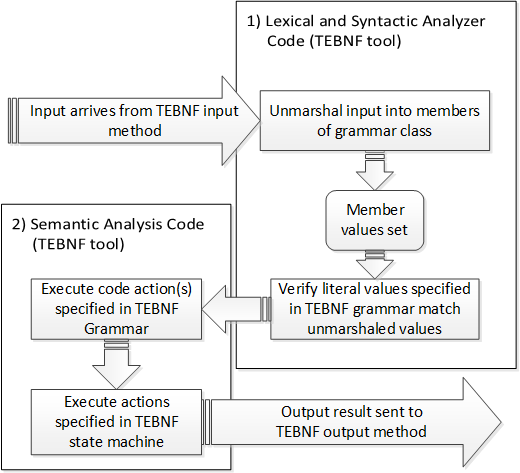
\includegraphics[width=0.9\textwidth]{figures/GeneratedCodeExecutionPath.png}
\caption{Execution path for code generated by the TEBNF code generation tool.}
\label{fig:GeneratedCodeExecutionPath}
\end{figure}

\indent
Grammar elements are translated by the prototype code generation tool into classes that serve a three-fold purpose.  Each grammar class can (1) unmarshal raw input data into specific user-defined types, (2) verify matches to byte patterns in the raw input data, and (3) marshal the values stored in the grammar class back into their original form and byte ordering.  Patterns in data arriving through TEBNF input methods are located by the state machine using unmarshal functions of grammar element classes.  As data arrives through an input method, patterns are recognized in the data by the grammar classes and simultaneously unmarshaled into the data types of those classes.  This means lexical analysis and parsing are performed in the same step, using a single TEBNF input (figure~\ref{fig:GeneratedCodeExecutionPath}).  This approach is different from traditional parser code generation methods.  Traditional methods require the use of a lexical analyzer generator tool and parser generator tool; each with their own input specification formats (see figure~\ref{fig:TraditionalCodeGenProcess}).

\section{State Machine and Actions Code Generation}
Path(s) of execution are defined in TEBNF using state machines, as shown in figure~\ref{fig:GeneratedCodeExecutionPath}.  State machines are represented in TEBNF using state transition table elements (see appendix~\ref{appendix:TEBNF}).  A state machine in TEBNF describes the order of tasks executed by a single application thread.  States are divided into a series of six steps.  These six steps are given below, in the order they are expressed in TEBNF, which is the same order they are evaluated by the generated code:
\begin{enumerate}
  \item A unique name that identifies the state and allows other states to reference it
  \item A Boolean condition that can be either a grammar to match with input data or an explicit Boolean condition.
  \item The method of input for receiving the input data (console, file, or UDP/IP).
  \item The next state to jump to if the Boolean condition provided in the second step evaluates to true.
  \item An output to send through the output method provided in the sixth step, an explicit code action to execute, or nothing.
  \item The output method to send output specified in the fifth step.  If an action or nothing was provided for the fifth step, then this step is empty as well.
\end{enumerate}

\indent
These state steps shape the way TEBNF elements interact with each other and input data by determining (1) what input methods data is received on, (2) what parts of the received data match defined grammar patterns, (3) what method is used to output that data, and (4) what code actions are executed.
 % Design
    \chapter{Implementing Tools with TEBNF}
This chapter focuses on the implementation of applications using TEBNF and the TEBNF code generation tool.  The chapter is divided into four sections.  The first section will showcase a real world example using a TEBNF grammar to parse data from a National Imagery Transmission Format (NITF) version 2.1 file.  The second section will walk through the implementation of two test cases.  The third section will cover the testing and verification of these test cases.  The fourth section of the chapter will cover the results of testing.

\section{NITF File Parsing: A Real World Example}
\label{sections:RealWorldNitfExample}
Software developers are oftentimes tasked to write software that parses and processes data in different formats.  A well-known example is word processing software.  Word processing software must be able to open and read documents structured in its own proprietary format and others (e.g. pdf, txt, etc.).  Creating software that reads specific data formats requires access to documentation detailing the exact structure of each format.

\indent
An example data format read by different applications is the NITF 2.1 file format.  The NITF 2.1 file format is part of a suite of standards established by the United States (US) Government for formatting digital imagery \cite{2500c_01}.  Documentation detailing the NITF 2.1 standard is freely available for download from the Geospatial Intelligence Standards Working Group’s website \cite{gwg_01}.  This file format is compatible with software used by members of the intelligence community, which includes the US Department of Defense (DoD) \cite{2500c_01}.  The VANTAGE\textsuperscript{TM} software suite produced by the Space Dynamics Laboratory and the SOCET Services suite produced by BAE Systems are all capable of reading and exploiting NITF 2.1 formatted files \cite{sdl_01,bae_01}.

\begin{figure}[htbp]
\centering
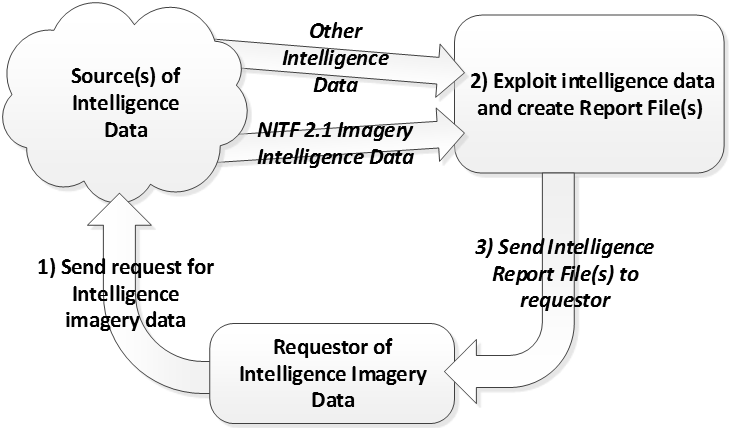
\includegraphics[width=0.9\textwidth]{figures/NitfConops.png}
\caption{Concept of operations for NITF 2.1 format files.}
\label{fig:NitfConops}
\end{figure}

\indent
As explained by \cite{2500c_01}, the stated purpose of the NITF 2.1 file format is to provide the intelligence community an interoperable means of transmission and/or storage of electronic imagery data.  The NITF 2.1 format is intended to be used in the dissemination of imagery derived intelligence data.  A general concept of operations involving NITF data is shown in figure~\ref{fig:NitfConops}.  First, imagery data in NITF 2.1 format is requested by a member of the intelligence community.  Second, the NITF data is received and combined with other collateral information to create intelligence report file(s) and/or products containing   the requested information of interest.  Third, these report files and/or products are given to the requestor of that intelligence information.

\indent
Exploiting NITF 2.1 files requires a detailed understanding of the format.  With this understanding, it is possible to create software than can parse NITF 2.1 files to find information of interest, generate report files, and/or products.

\indent
The NITF 2.1 file format is composed of a file header and one or more segments.  Each segment contains a subheader with data fields.  Each data field has a specific size and format (depending on the type of field) and is located at a specific byte offset within the file.

\indent
Conditional data and/or data characteristics can be added to NITF 2.1 files. This flexibility to extend the format is done using conditional fields in the file header and subheaders indicating the existence of Tagged Record Extensions (TREs) and Data Extension Segments.  Tagged Record Extensions contain data fields, while extension segments can contain data in new formats.

\begin{figure}[htbp]
\centering
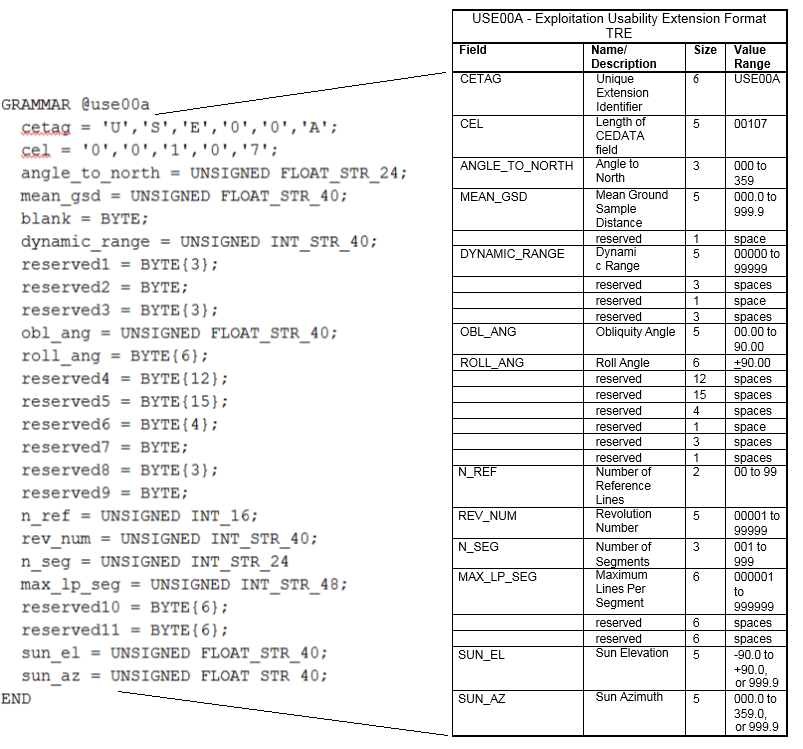
\includegraphics[width=0.9\textwidth]{figures/TreComparison.png}
\caption[TEBNF Implementation of the NITF 2.1 USE00A TRE]{TEBNF Implementation of the NITF 2.1 USE00A TRE (TRE information taken from \cite{use001_01}).}
\label{fig:tre}
\end{figure}

\indent
Gleaning data from NITF 2.1 formatted files for exploitation (see figure~\ref{fig:NitfConops}) is best achieved using applications that can read it.  Figure~\ref{fig:tre} demonstrates how this can be achieved using a TEBNF grammar.  The table shows a side-by-side comparison of the NITF 2.1 USE00A (Exploitation Usability Extension Format) TRE \cite{use001_01} compared to its equivalent implementation in TEBNF.  Each data field for this TRE is compared to its equivalent TEBNF grammar expression.  This comparison highlights several important advantages of using TEBNF to implement parsers of specifications like NITF:
\begin{itemize}
  \item Convenience.  There is no need to keep track of the offset of each data field because it is determined based on the size of each type.
  \item Readability.  TEBNF grammar syntax looks very similar to actual specifications as shown in figure~\ref{fig:tre}, making it is easier to understand.
  \item Self-documenting.  Since TEBNF grammar syntax ties the size of each data field to the size of the subelement type, the grammar helps to document itself. 
\end{itemize}

\section{Test Cases}
In order to verify the functionality of the TEBNF language, two case studies were implemented.  Both case studies showcase the strengths of TEBNF and the TEBNF code generation tool.  Further case studies are possible because TEBNF is Turing complete (see appendix~\ref{appendix:TEBNFTuringCompletenessProof}).

\subsection{Basic Calculator}
The first test case was to create a basic calculator console application that supports addition, subtraction, multiplication, and division of integers.  Producing this calculator required the tool to generate code that:
\begin{enumerate}
  \item Parses numeric data received over a console input.
  \item Makes calculations based on the data received from that console input.
  \item Sends the results of those calculations to console output.
  \item Allows the user to exit when finished.
\end{enumerate}

\indent
The calculator begins with a step executed once at the beginning of the program. This initial step prompts users to enter a number, which is then saved as an initial “result” value because all subsequent math operations are executed against it.  From this point onward, the calculator repeats a cycle that 1) asks for a number, 2) asks for a math operator, 3) applies that math operator against the saved result and the last number entered, 4) saves the result, and 5) displays that result.   This cycle then repeats until the user enters a ‘=’ operator, which then displays the result and exits the program.

\indent
Input for the calculator is achieved with a single TEBNF console input element containing two prompt values.  The first is used for prompting the user to enter a number, accepting a signed 64-bit integer.  The second one is used for prompting the user to enter a single character (math operator).  Outputting the result of math operations is accomplished with a single TEBNF console output element.

\indent
Acceptable input values for the calculator are limited to integers or one of five math operator characters (‘+’, ‘-‘, ‘*’, ‘/’, ‘=’).  TEBNF grammar elements are defined for each math operator.  Another grammar element was created to represent a signed 64-bit integer, providing a place to store integers as they are unmarshaled from input.  The saved result value is represented as a static variable within the number grammar element, serving as a place to store the result of each math operation.  An actions element was created for each of the supported math operators.  Each actions element adds, subtracts, multiplies, divides, or sets the saved result using the last unmarshaled integer.

\begin{figure}[htbp]
\centering
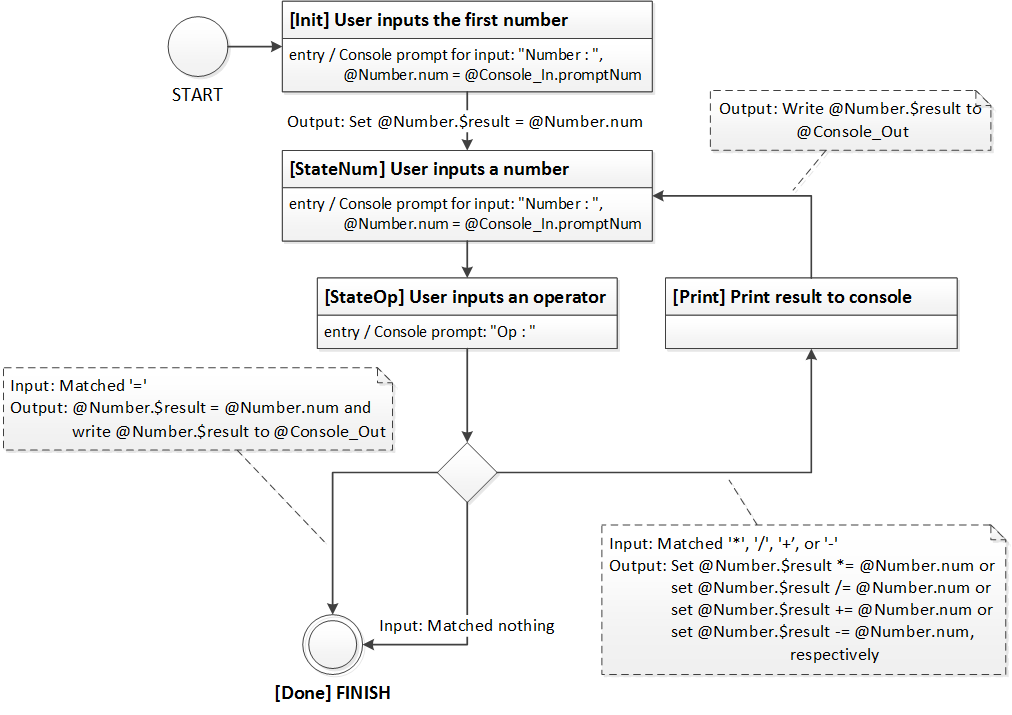
\includegraphics[width=0.9\textwidth]{figures/CalculatorUmlStateMachine.png}
\caption[State machine representing a calculator.]{State machine representing a calculator (includes pseudocode).}
\label{fig:CalculatorUmlStateMachine}
\end{figure}

\indent
The last TEBNF element included in the grammar describes the calculator as a state machine utilizing the elements described above to define the execution path of the calculator.  The TEBNF grammar that implements this calculator is provided in listing~\ref{ExampleCalculator}.

\indent
The calculator state machine is represented with five states, as shown in figure~\ref{fig:CalculatorUmlStateMachine}.  The first state of the machine is a special case entered only once at the beginning of execution.  This initial state is a necessary special case that sets the ongoing result value for subsequent math operations.  In this state the user is prompted to enter the initial number via the console input element.  The number grammar element unmarshals this input value as a signed 64-bit integer and retains a copy for later use.  The state table then executes an actions element.  This actions element sets the result static variable equal to the unmarshaled value while the machine transitions to the next state.

\indent
After setting the result value while transitioning to the first state of the main cycle, the machine uses the console input element to prompt the user to enter a number again.  This number is also unmarshaled from input and stored as before.  The state machine then transitions to the next state.

\indent
This state uses the console input element to prompt the user to enter one of the supported math operators.  The state machine does this by moving through a series of “else-if” states.  Each state uses one of the math operator grammar elements to check the same console input for a match to one of the supported math operations.  A match occurs when a grammar successfully unmarshals the input value.  Upon matching an operator the machine transitions to the print state and executes an actions element applying that operator to the result and unmarshaled number, then assigns it to the result.  As the print state transitions to the first state of the main cycle, an actions element is executed that writes the result to the console.  The cycle then continues to repeat until the user enters a '=' to exit.  Otherwise, if a '=' operator was matched, the result is written to the console as the state machine transitions to the done state.  If the input matched nothing, the state machine transitions to the done state.

\begin{table}[h]
\begin{center}
\caption{Sample input and output data for the calculator.}
\label{sampleCalculatorIoData}
\begin{tabular}{|l|l|l|} \hline
\textbf{Operand} & \textbf{Operator} & \textbf{Result} \\
\hline \hline
5	& \cellcolor{gray!25} & \cellcolor{gray!25} \\ \hline
10	& +	& 15    \\ \hline
95	& -	& -80   \\ \hline
110	& +	& 30    \\ \hline
10	& /	& 3     \\ \hline
111	& *	& 333   \\ \hline
33	& -	& 300   \\ \hline
20	& /	& 15    \\ \hline
5	& *	& 75    \\ \hline
0   & = & 75    \\
\hline                                  
\end{tabular}
\end{center}
\end{table}

\indent
Suppose this calculator is run using the sample data in table~\ref{sampleCalculatorIoData}.  The first line in the table is the initial value 5.  The second operand entered by the user is the number 10.  The '+' operator is entered by the user, and the result displayed is 15.  Entering the next value of 95 followed by the operator '-' displays the number -80.  This cycle continues until the user enters the '='  operator.

\subsection{NITF 2.1 UDP/IP File Transfer Client}
The second test case is a file transfer client that receives NITF 2.1 files over UDP/IP upon requesting them from a file server.  The server tells the client when it is done sending files so the client knows when to exit.  This requires the tool to generate code for a file client that:
\begin{enumerate}
  \item Asks the server to send it a file by sending it a message over a UDP/IP output.
  \item Receives the NITF 2.1 file from the server over a UDP/IP input.
  \item Uses the file length data field in the NITF 2.1 file to determine that it has received the entire file from the server as it was sent over UDP/IP.
  \item Writes that file to disk using a file output.
  \item Quits upon receiving a message from the server that says it is done sending files.
\end{enumerate}

\indent
The NITF 2.1 file transfer client starts by prompting the user to enter the IP address and port that will be used for sending and receiving data over UDP/IP.  After entering this information, the client immediately sends the message "“send”" to the server to request that it send a file.  Once the server receives the "“send"” message from the client, it reads a NITF 2.1 file from disk and begins sending it to the client over UDP/IP.  As the client receives data from the server, it continually checks to see if it has received the entire NITF 2.1 file from the server.  The client knows a file transfer is complete when it has received the amount of data specified in the NITF file’s file length data field.  The client then prompts the user to enter a path including the file name specifying where the file will be written to disk.  After writing the file to disk, the client requests the next file from the server.

\indent
Allowed input values for the client are limited to a string for the IP address, an unsigned integer for the port, and strings for file paths.  All other input to the client comes from the server through a TEBNF UDP/IP input element.  A UDP/IP output element is used by the client to send data to the server.  One file output element is used by the client for writing files to disk received from the server.

\indent
A grammar element was created to find NITF 2.1 files in data received over UDP/IP.  The beginning of each NITF 2.1 file can be found by searching for the byte sequence "NITF02.10", which is always found at the beginning of each file.  The NITF 2.1 file header has a data field containing the length of the file.  This is leveraged by the TEBNF grammar element to calculate the end offset of each file.   A second grammar element was created for finding the "“done”" message in incoming data.  A third grammar was created to define the send message.  The TEBNF grammar that implements this file transfer client is provided in listing~\ref{ExampleUDPNitfReceiver}.

\begin{figure}[htbp]
\centering
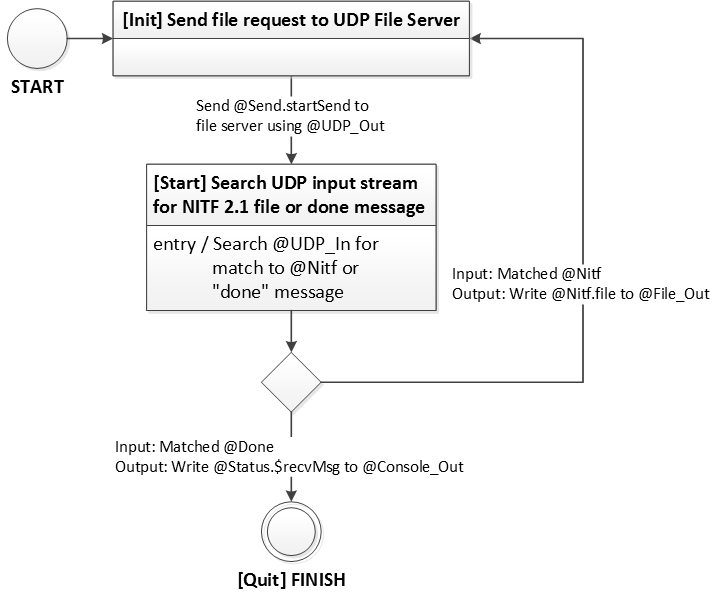
\includegraphics[width=0.9\textwidth]{figures/NitfFileClientUmlStateMachine.png}
\caption[State machine representing a NITF 2.1 UDP/IP file transfer client]{State machine representing a NITF 2.1 UDP/IP file transfer client (includes pseudocode).}
\label{fig:NitfFileClientUmlStateMachine}
\end{figure}

\indent
The file transfer client can be represented as a state machine with three states, as shown in figure~\ref{fig:NitfFileClientUmlStateMachine}.  While transitioning from the first state to the second, the “send” message is sent via the UDP/IP output element to the file server.

\indent
The second state looks at data received from the file server over the UDP/IP input element to determine if it contains a NITF 2.1 file or the "“done”" message.  If the incoming data contains a NITF file, the state machine writes it to the file output element while transitioning to the back to the first state which tells the server to send the next file, which prompts the user for a path to write the file to.  The state machine then transitions back to the first state which tells the server to send the next file.  If the incoming data does not contain a file, an "“else-if”" case in this same state checks for the “done” message.  If the done message was received, the machine writes a message to the console output telling the user that all files have been received, after which the machine transitions to the quit state and exits.

\indent
In a hypothetical case, assume there are five NITF 2.1 files to be sent to a test case file client.  Each file has a specific file size, as shown in table~\ref{sampleNitfSizeServerData}.

\begin{table}[h]
\begin{center}
\caption{Sizes of sample NITF 2.1 files sent to the test client.}
\label{sampleNitfSizeServerData}
\begin{tabular}{|c|} \hline
\textbf{NITF 2.1 File Size (bytes)} \\ \hline \hline
828710 \\ \hline
4021118 \\ \hline
912294 \\ \hline
3516054 \\ \hline
998822 \\ \hline                                  
\end{tabular}
\end{center}
\end{table}

\indent
The NITF 2.1 file server would be started and begin listening on its UDP/IP socket for the "send" request from a client.  The test case file client is then started and immediately sends a "send" request to the server, and a file transfer begins.  The UDP server reports the size in bytes of each file sent.  The file client writes each file to local disk.  The size in bytes of each file received corresponds to the size the files sent by the server.

\section{Results}
C++ code was successfully generated by the TEBNF code generation tool for each of the test cases.  The TEBNF code generation tool provides useful output when it generates code from a supplied input grammar.  The tool displays information  indicating when each stage of the code generation process finishes.  Status for the generation stage displays the classes generated for each element.  After the  generation stage finishes and all of the code has been generated, the tool reports success and the number of element files generated.  Console output from generating code for the calculator test case and the NITF 2.1 file client test case is shown in figures~\ref{fig:TestCaseBuildCalculator} and ~\ref{fig:TestCaseBuildNitfReceiver}.

\begin{figure}[h!]
\centering
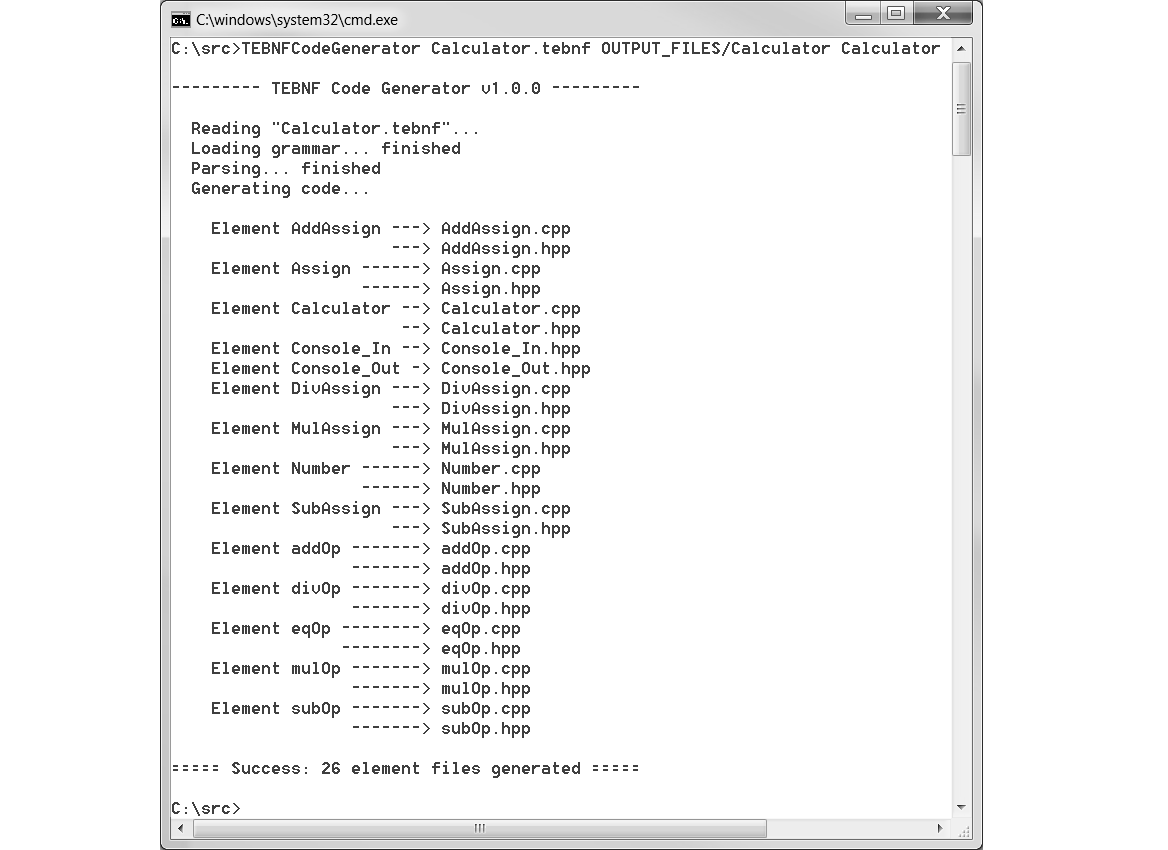
\includegraphics[width=0.9\textwidth]{figures/TestCaseBuildCalculator.png}
\caption{TEBNF code generation tool output for the calculator test case.}
\label{fig:TestCaseBuildCalculator}
\end{figure}

\begin{figure}[h!]
\centering
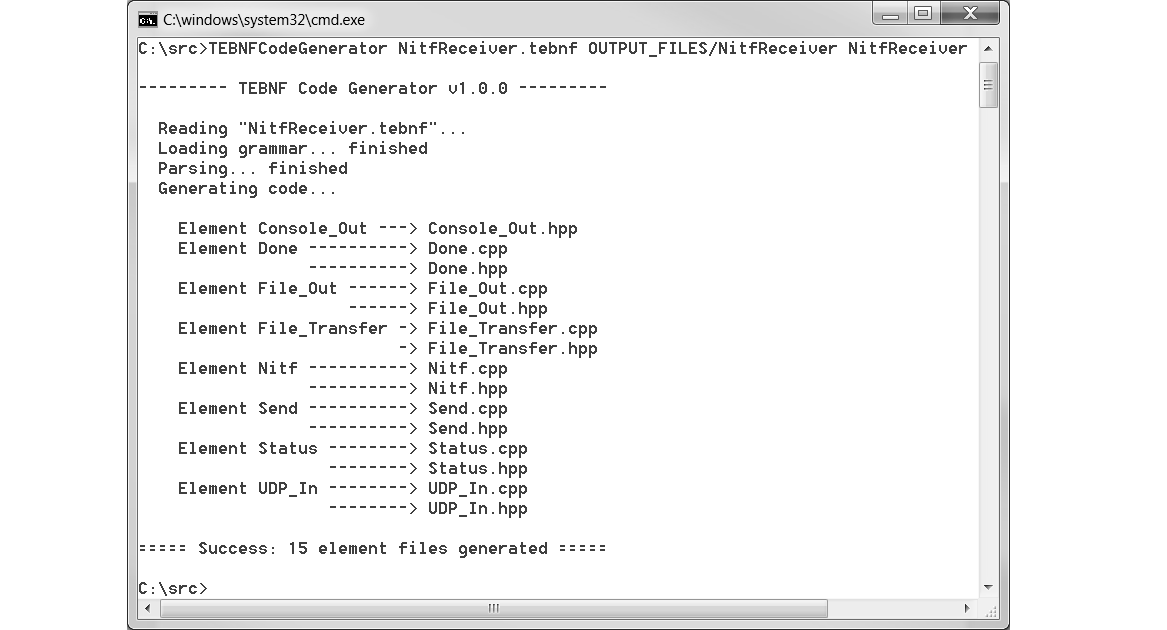
\includegraphics[width=0.9\textwidth]{figures/TestCaseBuildNitfReceiver.png}
\caption{TEBNF code generation tool output for the UDP NITF 2.1 file client test case.}
\label{fig:TestCaseBuildNitfReceiver}
\end{figure}

\indent
A CMakeLists.txt file was correctly generated by the TEBNF code generation tool for each test case, and CMake version 3.0.2 was run using those CMakeLists files to generate Microsoft Visual Studio 2013 solution and project files.  The project files generated by CMake for both test cases were successfully opened and built in Microsoft Visual Studio 2013.

\subsection{Calculator}
\label{subsections:GeneratedCalculator}
The calculator test case executable was run using the test data from table~\ref{sampleCalculatorIoData}.  As expected, the input and output of the calculator (figure~\ref{fig:TestCaseRunCalculator}) matched what is defined in table~\ref{sampleCalculatorIoData}.  This means the behavior of the calculator test case matches the behavior defined in the TEBNF grammar it was generated from.

\begin{figure}[h!]
\centering
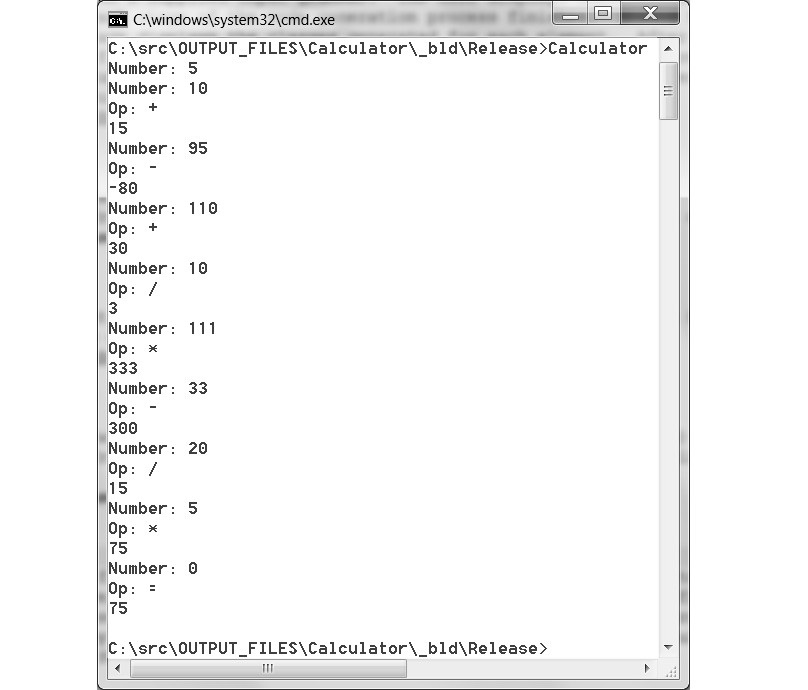
\includegraphics[width=0.9\textwidth]{figures/TestCaseRunCalculator.png}
\caption{Running the calculator test case.}
\label{fig:TestCaseRunCalculator}
\end{figure}

\subsection{NITF 2.1 File Client}
\label{subsections:GeneratedFileClient}
The NITF 2.1 file client test case executable was run using the five sample NITF 2.1 files whose sizes are found in table~\ref{sampleNitfSizeServerData}.  A NITF 2.1 file server was created that listened for client "send" requests over a UDP/IP socket on localhost port 10042.  This server was started, then the test case client was started and configured to send requests and receive file transfers on localhost port 10042.  The expected outcome occurred, with the server successfully sending five files as indicated by the first five send messages output by the server in figure~\ref{fig:TestCaseRunNitfServer}.  This was followed by the last four byte "done" message is sent to notify the client it was done sending.  The same five files were received by the client which prompted for a file name to save each file as shown in  figure~\ref{fig:TestCaseRunNitfReceiver}.  After saving the files, the client exited because the server had sent the "done" message.

\begin{figure}[h!]
\centering
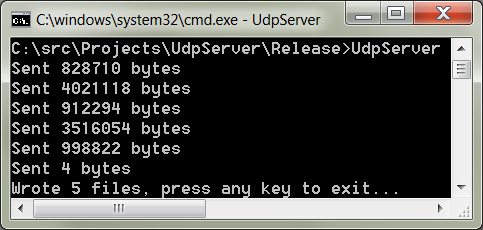
\includegraphics[width=0.9\textwidth]{figures/TestCaseRunNitfServer.png}
\caption{Running the file server for the NITF 2.1 file client test case.}
\label{fig:TestCaseRunNitfServer}
\end{figure}

\begin{figure}[h!]
\centering
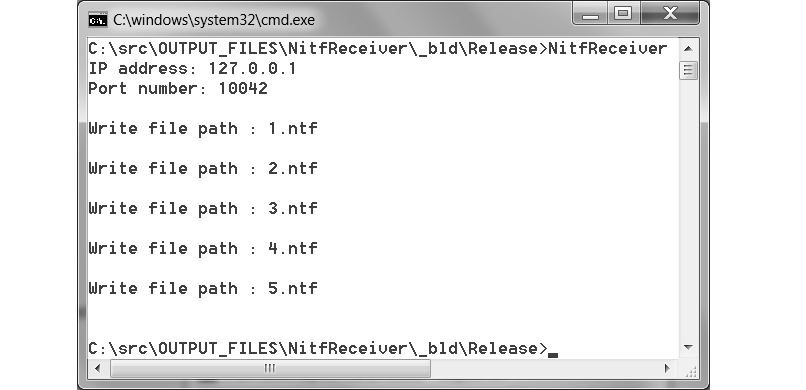
\includegraphics[width=0.9\textwidth]{figures/TestCaseRunNitfReceiver.png}
\caption{Running the NITF 2.1 file client test case.}
\label{fig:TestCaseRunNitfReceiver}
\end{figure}

\indent
The sizes of the files received were an exact match to the file sizes listed in table~\ref{sampleNitfSizeServerData}, as the output of the server and client test case executables show in figures~\ref{fig:TestCaseRunNitfServer} and~\ref{fig:TestCaseRunNitfReceiver}, respectively.  This verifies that the behavior of the NITF 2.1 client test case matches the behavior defined in the TEBNF grammar it was generated from.

\section{Comparing C++ to TEBNF}
\label{sections:ComparingCplusplusToTEBNF}
A non-generated C++ implementation of each test case was also written.  The state machines described in chapter~\ref{chapters:Design} for both test cases served as the starting point of each implementation.  Using the same design as the generated test cases, a baseline was established for more direct comparisons.

\subsection{Test Case Experience}
The non-generated C++ implementation of both test cases was verified by following the procedures outlined in subsections~\ref{subsections:GeneratedCalculator} and~\ref{subsections:GeneratedFileClient}.  Each was verified to have the same behavior and output as the test cases generated from TEBNF.

\indent
The TEBNF grammar for each test case was significantly shorter than its manual C++ counterpart.  The non-generated C++ implementations had fewer lines of code than their counterparts generated from TEBNF.  These results were expected because the TEBNF code generation tool does not yet perform optimization.

\indent
Writing code to handle I/O and input verification took longer in C++ than TEBNF, which only requires a declaration to setup any of the supported I/O methods.  Though this inconvenience was observed while writing the calculator test case in C++, it was far more noticeable while writing the client.  The client uses three different I/O methods whereas the calculator only uses one.  It is evident that a more complicated application can be more convenient to write in TEBNF than C++.  The time it took to implement both test cases in C++ and TEBNF are listed in tables~\ref{calcImplementationTimes} and~\ref{testCaseNitfRecvTimes}.

\begin{table}[h]
\begin{center}
\caption[Calculator Test Case Implementation Times]{Calculator Test Case Implementation Times (measured in hours).}
\label{calcImplementationTimes}
\begin{tabular}{|c|c|c|} \hline
\textbf{Item to Implement} & \textbf{C++} & \textbf{TEBNF} \\ \hline \hline
Console I/O                & 1            & 0.1            \\ \hline
State Machine              & 1            & 0.5            \\ \hline
\textbf{Total}             & \textbf{2}   & \textbf{0.6}   \\ \hline
\end{tabular}
\end{center}
\end{table}

\begin{table}[h]
\begin{center}
\caption[NITF File Client Test Case Implementation Times]{NITF File Client Test Case Implementation Times (measured in hours).}
\label{testCaseNitfRecvTimes}
\begin{tabular}{|c|c|c|} \hline
\textbf{Item to Implement} & \textbf{C++} & \textbf{TEBNF} \\ \hline \hline
Console I/O                & 1            & 0.1            \\ \hline
File I/O                   & 1            & 0.1            \\ \hline
UDP/IP I/O                 & 4            & 0.5            \\ \hline
State Machine              & 4            & 1              \\ \hline
\textbf{Total}             & \textbf{10}  & \textbf{1.7}   \\ \hline
\end{tabular}
\end{center}
\end{table}

\indent
Another disparity in coding effort was observed while writing the NITF file parser in C++.  Creating NITF parsing code in C++ took a lot more effort than in TEBNF.  The non-generated implementation required calculation of an offset whenever it was necessary to jump to a specific location in the NITF file.  Calculation of this offset requires knowledge beforehand of the size and position of each field.  On top of this, fields in the NITF standard can vary in length and be of different formats, as explained in section~\ref{sections:RealWorldNitfExample}.  Compare this effort to the TEBNF implementation found in listing~\ref{ExampleUDPNitfReceiver} which made it possible to write a parser resembling the actual specification document itself.

\subsection{Test Case Analysis}
A widely accepted metric for measuring code complexity is McCabe's Cyclomatic Complexity \cite{cardoso_01}.  This metric was derived from graph theory by McCabe to measure the number of control flow paths in a code module \cite{cardoso_01}.  McCabe's Cyclomatic Complexity is $ e - n + 2 $, where $e$ is the number edges in the control flow graph and $n$ is the number of nodes \cite{cardoso_01}.  An example of its use proposed by \cite{zhang_01} employs McCabe's Cyclomatic Complexity metric to effectively predict defects in code modules.

\indent
The Lizard code complexity analyzer \cite{lizard_01} tool was used to analyze each test case.  The analysis results from the tool contained several valuable metrics, including the average cyclomatic complexity number (CCN) \cite{lizard_01} of every function in the test cases.  The analysis results of each test case are provided in tables~\ref{LizardAnalysisFileClient} and \ref{LizardAnalysisCalculator}.  Values related to the interquartile range (IQR) were calculated from the analysis data of each test case, including the lower (first) quartile (Q1) corresponding to the $25^{th}$ percentile, the higher quartile (Q3) corresponding to the $75^{th}$ percentile, and the median.  In order to focus on the most relevant analysis data, the upper limit ($U_{CCN}$) and lower limit ($L_{CCN}$) of each data set was calculated as $Q3 + 1.5(IQR)$ and $Q1 - 1.5(IQR)$, respectively.

\begin{table}[h]
\begin{center}
\caption{Analysis results for the NITF file client test cases.}
\label{LizardAnalysisFileClient}
\begin{tabular}{|l|c|c|c|c|} \hline
\textbf{Test Case} & \textbf{Avg. CCN} & $\mathbf{U_{CCN}}$ & \textbf{Avg. Token Count} & \textbf{Func. Count} \\ \hline \hline
Generated     & 2.00 & 3 & 54.49  & 136 \\ \hline
Non-generated & 3.38 & 6 & 101.81 & 16  \\ \hline
\end{tabular}
\end{center}
\end{table}

\begin{table}[h]
\begin{center}
\caption{Analysis results for the calculator test cases.}
\label{LizardAnalysisCalculator}
\begin{tabular}{|l|c|c|c|c|} \hline
\textbf{Test Case} & \textbf{Avg. CCN} & $\mathbf{U_{CCN}}$ & \textbf{Avg. Token Count} & \textbf{Func. Count} \\ \hline \hline
Generated     & 1.89 & 3 & 49.50 & 135 \\ \hline
Non-generated & 3.42 & 7 & 81.42 & 12  \\ \hline
\end{tabular}
\end{center}
\end{table}

\indent
The data in tables~\ref{LizardAnalysisFileClient} and \ref{LizardAnalysisCalculator} show differences between the generated and non-generated test cases.  Compared to the non-generated C++ implementations, the test cases generated from TEBNF have (1) more functions, (2) a lower average number of tokens per function, and (3) a lower average CCN per function.

\begin{table}[h]
\begin{center}
\caption{P-values calculated from the analysis data of each test case.}
\label{LizardAnalysisPvalues}
\begin{tabular}{|l|c|c|} \hline
\textbf{Test Case} & $\mathbf{P_{CCN}}$ & $\mathbf{P_{TokenCount}}$ \\ \hline \hline
File Client & 0.041236 & 0.007916 \\ \hline
Calculator  & 0.017212 & 0.043956 \\ \hline
\end{tabular}
\end{center}
\end{table}

\indent
Analysis data for the generated and non-generated test cases look similar but are provably different.  Table~\ref{LizardAnalysisPvalues} shows the p-values calculated for the test cases.  All of the p-values are significant at p $<$ 0.05, supporting the hypothesis that the data sets are different.

\begin{figure}[h!]
\centering
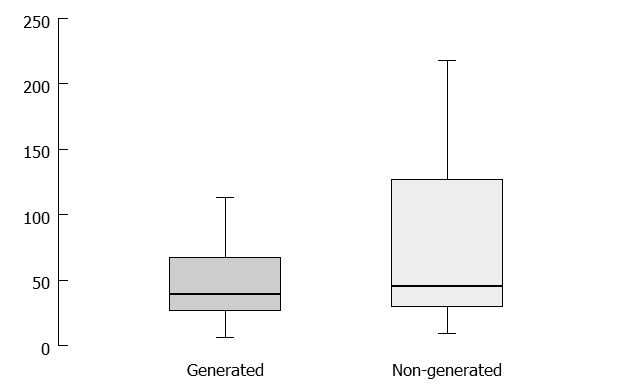
\includegraphics[width=0.9\textwidth]{figures/Lizard_FileClient_TokenCount.png}
\caption[Box plot of function token count for the file client test cases.]{Box plot of function token count for the file client test cases (omits outliers).}
\label{fig:Lizard_FileClient_TokenCount}
\end{figure}

\begin{figure}[h!]
\centering
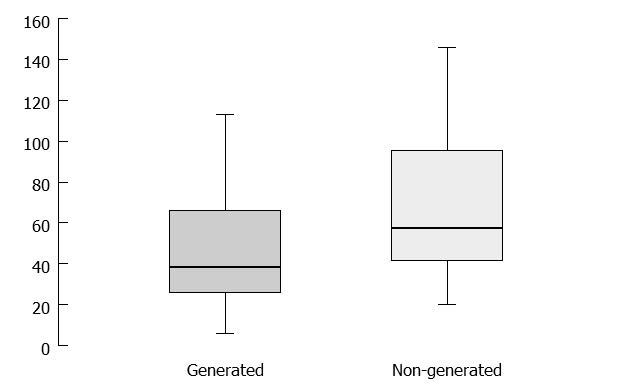
\includegraphics[width=0.9\textwidth]{figures/Lizard_Calculator_TokenCount.png}
\caption[Box plot of function token count for the calculator test cases.]{Box plot of function token count for the calculator test cases (omits outliers).}
\label{fig:Lizard_Calculator_TokenCount}
\end{figure}

%\indent
%The difference in the number of functions between implementations is due to the fact %that code generated from TEBNF splits up larger computational problems into smaller %tasks than the non-generated implementations.  This dividing of tasks yields more %functions, leading to a need to combine logical groupings of functions into classes.

\indent
Tables~\ref{LizardAnalysisFileClient} and \ref{LizardAnalysisCalculator} show that the generated code has a lower average token count per function than the non-generated code.  Figures~\ref{fig:Lizard_FileClient_TokenCount} and \ref{fig:Lizard_Calculator_TokenCount} graphically support the assumption that the generated code averages a lower number of tokens per function.  The first conclusion to be drawn from the data as plotted in these figures is that larger computational problems are being split into smaller tasks.  This conclusion can be drawn based on the fact that lower median values within smaller data spreads point to a greater number of functions with lower token counts. 

\indent
In the end, the lower average CCN for generated code (tables~\ref{LizardAnalysisFileClient} and \ref{LizardAnalysisCalculator}) is the strongest indicator that larger computational problems are being broken down into smaller ones.  Figures~\ref{fig:Lizard_FileClient_CCN} and \ref{fig:Lizard_Calculator_CCN} show that the median CCN for the generated test cases are at or below the lowest values measured for the non-generated test cases.

\indent
The main conclusion to be drawn is that lower token counts and CCN values in code generated from TEBNF both point to a trend in the data showing it is less error-prone than the non-generated code.  This conclusion is supported by fact that \cite{zhang_01} was able to use CCN values to detect the presence of defects in code.

\begin{figure}[h!]
\centering
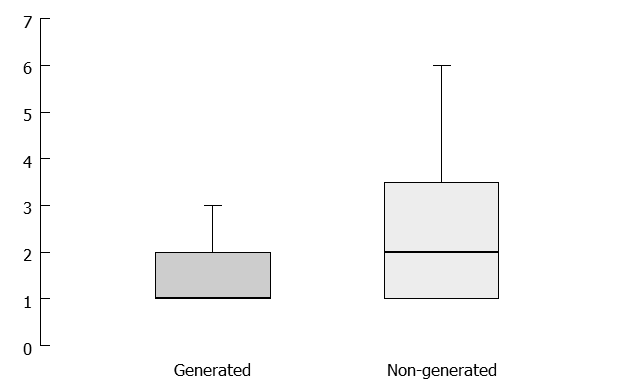
\includegraphics[width=0.9\textwidth]{figures/Lizard_FileClient_CCN.png}
\caption{Box plot of function cyclomatic complexity (CCN) for the file client test cases.}
\label{fig:Lizard_FileClient_CCN}
\end{figure}

\begin{figure}[h!]
\centering
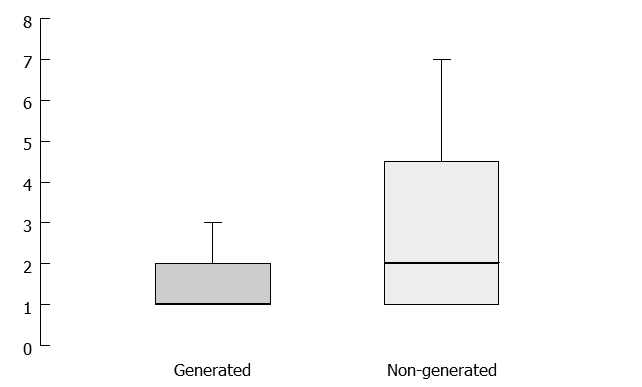
\includegraphics[width=0.9\textwidth]{figures/Lizard_Calculator_CCN.png}
\caption{Box plot of function cyclomatic complexity (CCN) for the calculator test cases.}
\label{fig:Lizard_Calculator_CCN}
\end{figure}






 % Implementation
    \chapter{Future Work}
Code generation using TEBNF creates several areas for future work.
\begin{itemize}
  \item Additional IO methods.  Some of these could include support for TCP/IP, MySQL databases, and others.
  \item A TEBNF Integrated Development Environment (IDE).  The IDE could provide intelligent code completion or incorporate a drag-and-drop interface for adding TEBNF elements to a grammar.
  \item Aspect oriented code generation.  This could involve generating code that leverages aspects.  It could also involve the integration of aspects into the specification of TEBNF itself.
  \item Exploring the use of template meta-programming in generated C++ code.  This programming paradigm emphasizes the use of types, similar to TEBNF.
  \item Software Mining for Graphical User Interface (GUI) code generation \cite{kennard_01,kennard_02}.  TEBNF lends itself to automatic generation of GUI code because of its merging of different input specifications into one.   Kennard proposed the usage of a technique called runtime data mining to generate GUIs \cite{kennard_01}.  Software mining \cite{kennard_02} is a form of data mining that focuses on the inspection of software information characteristics:
  \item Static characteristics: e.g. source code files and database schemas.
  \item Runtime characteristics: e.g. polymorphic data-types, other data values, reading and modification of an instantiated object’s current state.
\end{itemize} % Future work
    \chapter{Conclusion}
TEBNF merges the strengths of declarative and imperative programming paradigms into one format.  A prototype code generation tool was presented that accepts a TEBNF grammar as its sole input specification.  The prototype code generation tool demonstrated how TEBNF makes it possible to:
\begin{itemize}
  \item Integrate lexical analysis and parsing input specifications into one format.
  \item Generate C++ classes that handle IO over console, file, or UDP/IP, and abstract the complexities of their usage through TEBNF.
  \item Generate C++ classes that simultaneously unmarshal and match incoming input data to TEBNF grammar patterns.
  \item Describe the execution path of an application that accepts input over various IO methods, is able to parse that input, use it, and send output over various IO methods.
\end{itemize}

\indent
Software developers using TEBNF are able to focus on what they want to implement rather than how to represent their designs in a language like C++.  TEBNF embodies the idea of using additional levels of indirection to solve problems in computer science.
 % Conclusion
    
    % Endmatter
    \references{report}{USU-IEEEtran}
    
    \makeappendices
\appendix{TEBNF Syntax and Usage}
\label{appendix:TEBNF}

\appendixsection{TEBNF Grammar Syntax}
\label{sec:TEBNFGrammarSyntax}
Like standard EBNF, Typed EBNF (TEBNF) is used to express a context-free grammar that consists of non-terminal production rules and terminal symbols that may or may not have a type.  The typing of terminal symbols makes it possible to describe exactly how the input is recognized, yet preserves the simple syntax of EBNF.  TEBNF provides a set of input and output methods, grammar rules, and actions, tied together to a set of states using a state transition table.  It allows users to:
\begin{itemize}
  \item Describe how the input data will be sent to the generated application (UDP, file, or in-memory).
  \item Describe when and how responses will be sent to the sender as needed by the specified protocol.
  \item Describe what the input data sent to the generated application will look like.  This combines the traditional specification of lexical and syntactic analysis.
  \item Describe how the data will be processed by the generated application after the lexical and syntactic analysis stage.
  \item Describe the expected output of the application after it has been processed.  
  \item Leverage existing knowledge of EBNF grammars rather than require the learning of a completely new format.
\end{itemize}

\appendixsection{TEBNF Structure}
\label{sec:TEBNFStructure}
The structure of TEBNF is composed of a set of elements.  There are five kinds of elements in TEBNF: input methods, output methods, grammar sections, actions, and state transition tables.  Collectively, these elements and their contents are known as a TEBNF grammar.  Each TEBNF grammar requires at least one or more of each kind of element.

\appendixsection{TEBNF Elements and Subelements}
\label{sec:TEBNFElementsAndSubelements}
TEBNF elements (table~\ref{TEBNFElements}) contain one or more subelements.  Subelements within TEBNF consist of production rules, typed terminals, non-typed terminals, literal values, operators, states, and static variables.

\begin{table}[h!]
\begin{center}
\caption{TEBNF Elements.}
\label{TEBNFElements}
\begin{tabular}{|l|l|} \hline
\textbf{Element} & \textbf{Description} \\ \hline \hline
INPUT @name & specifier	Input element of a specific input specifier. \\ \hline
OUTPUT @name & specifier	Output of a specific output specifier. \\ \hline
GRAMMAR @name & Start of grammar section. \\ \hline
ACTIONS @name & Contains one or more actions. \\ \hline
STATES @name & Start of state transition table section. \\ \hline
END	& End of element section. \\ \hline
\end{tabular}
\end{center}
\end{table}

\indent
Subelements are declared where they are first used.  TEBNF infers what a subelement is by the way it is used.  Each element requires a name be given to it.  Element names are case-sensitive, can only contain visible characters, and are always prefixed by the '‘@'’ character as shown in example~\ref{ExampleElementName}:

\begin{equation}
GRAMMAR \ @packet
\label{ExampleElementName}
\end{equation}

\appendixsection{TEBNF Scoping Rules}
\label{sec:TEBNFScopingRules}
Elements and subelements are directly accessible at the scope they are created, similar to the C++ language.  Elements can be declared within the scope of other elements.  Subelements exist within the scope of their respective elements.  Each type of element has specific types of subelements that can be declared only within the scope of that type of element.

\appendixsection{TEBNF Types}
\label{sec:TEBNFTypes}
Association of types (table~\ref{TEBNFSymbols}) with terminal symbols offers an extra level of precision when matching specific patterns found in input data.  These symbols are called typed terminals.  TEBNF can infer the type of a terminal symbol because each type has two important components.

\begin{table}[h!]
\begin{center}
\caption{TEBNF symbols, production rules, non-typed terminals, and typed terminals.}
\label{TEBNFSymbols}
\begin{tabular}{|l|l|l|} \hline
\textbf{Type} & \textbf{Description} & \textbf{Example} \\ \hline \hline
symbol & Production rule  & alphabet \\
       &(non-terminal)    &          \\ \hline
symbol & Non-typed terminal   & '‘a'’, '‘b’', '‘c'’, 0xAB, \\
       & (1 or more literals) & “"String literal"”     \\ \hline                    
\#comment & Single-line comment & \#This is a comment. \\ \hline
\#\#      & Multi-line comment & \#\# This is a really,   \\
comment &                    & really, really long    \\
\#\#      &                    & multi-line comment. \#\# \\ \hline
\$var & Static variable & \$myValue = 42 ; \\ \hline
type & Typed terminal & CHAR\{0,\} ; \\ \hline
%BIT & Represents 1 bit & My\_Byte = BIT\{8\} ; \\ \hline
BYTE & Represents a & My\_Kb = BYTE\{1024\} ; \\
     & 8-bit byte	&                       \\ \hline
INT\_X      & Represents an integer & My\_Int = INT\_64; \\
            & of size X bits        &                  \\ \hline
INT\_STR\_X & Represents an integer & fileLength = UNSIGNED \\
            & as a string of size   & INT\_STR\_96;         \\           
            & X bits                &                       \\ \hline
CHAR        & Represents a 8-bit    & MyChar = CHAR ;        \\
            & character             & MyString = CHAR\{128\} ; \\ \hline
FLOAT\_X    & Floating-point number & MyFloat = FLOAT\_64 ; \\
            & of size X bits        &                      \\ \hline
UNSIGNED    & Unsigned number & UNSIGNED INT\_16\{2\} ; \\
            & terminal        &                      \\ \hline
\end{tabular}
\end{center}
\end{table}

\indent
First, each type has an inherent size in bits or bytes.  Whenever data is matched to a specific type the size is immediately known.  Because the size of each type is known beforehand, the offset of the next symbol is immediately known.  Second, each type inherently identifies how it should be used in a given context.  TEBNF types are expressed by assigning a type to a terminal production symbol, as shown in example~\ref{ExampleTypeAssignment}:

\begin{equation}
payload\ =\ INT\_64
\label{ExampleTypeAssignment}
\end{equation}

\indent
TEBNF also has static variables, which are a kind of subelement that can assume the type of whatever is assigned to them.  They are static because they have global visibility$-$i.e. they can be declared anywhere and accessed from any other element, regardless of where they were declared.  Static variables are always prefixed by the '‘\$'’ character (example~\ref{ExampleStaticVariableAssignment}):

\begin{equation}
\$payloads\ =\ payload
\label{ExampleStaticVariableAssignment}
\end{equation}

\indent
A static variable can become typed when a typed terminal is assigned to it.  Production rules, terminals, and literals can also be assigned to static variables.  This capability makes static variables the most flexible subelement available in TEBNF.

\appendixsection{TEBNF Operators}
\label{sec:TEBNFOperators}
There are three categories of operators in TEBNF.  First are production rule operators (table~\ref{TEBNFProductionRuleOperators}), which are used to build production rules.  Second are arithmetic and comparison operators (table~\ref{TEBNFArithmeticAndComparisonOperators}).  Arithmetic and comparison operators are a key difference between TEBNF and standard EBNF, which does not have them.  Third is inter-element operators that perform operations on and/or between elements (table~\ref{TEBNFInterElementOperator}).  The only operator that falls in this category is the "AS" operator.

\begin{table}[h!]
\begin{center}
\caption{TEBNF production rule operators.}
\label{TEBNFProductionRuleOperators}
\begin{tabular}{|l|l|l|} \hline
\textbf{Operator} & \textbf{Description} & \textbf{Example} \\ \hline \hline
=   & Definition$—$i.e. & alphaNumericCharacter \\
    & is defined as     & = letter $|$ number ;  \\ \hline
=   & Grammar total     & = fileLength ; \\
    & length            &                \\ \hline
,   & Concatenation	    & twoLetters =      \\
    &                   & letter , letter ; \\ \hline
;   & Termination       & twoVals =    \\
    &                   & val1, val2 ; \\ \hline
$|$   & Or	            & letter $|$ number \\ \hline
$|$   & State Transition  & Start $|$ packet $|$ … \\
    & table delimiter   &                    \\ \hline
.   & Element member    & @packet.payloadSize \\
    & access            &                     \\ \hline
%(…) & Sub-rule Closure	& (letter) \\ \hline
\{min,max\} & Occurrence range & letter\{0,\} \\ \hline
{len}     & Exact range,  & letter\{26\} \\
          & where len is  &            \\
          & the min and   &            \\
          & max.          &            \\ \hline
[\ ]      & Array subscript	& myChar[5] \\ \hline
\end{tabular}
\end{center}
\end{table}

\begin{table}[h!]
\begin{center}
\caption{TEBNF arithmetic and comparison operators.}
\label{TEBNFArithmeticAndComparisonOperators}
\begin{tabular}{|l|l|l|} \hline
\textbf{Operator} & \textbf{Description} & \textbf{Example} \\ \hline \hline
== & Equality & \$X == \$Y \\ \hline
=  & Assign   & \$x = 45 ; \\ \hline
+  & Add      & \$x = \$y + \$z \\ \hline
-  & Subtract & \$x = \$g - \$h \\ \hline
+= & Addition assignment & 	 \\ \hline
++ & Post-increment &  \\ \hline
-= & Subtraction assignment &  \\ \hline
-- & Post-decrement &  \\ \hline
*  & Multiply & \$x = \$y * 92 \\ \hline
/  & Divide & X = 1 + (y – 2) \\ \hline
\end{tabular}
\end{center}
\end{table}

\begin{table}[h!]
\begin{center}
\caption{TEBNF inter-element operator.}
\label{TEBNFInterElementOperator}
\begin{tabular}{|l|l|l|} \hline
\textbf{Operator} & \textbf{Description} & \textbf{Example} \\ \hline \hline
AS & Defines a new    & OUTPUT @UDP\_Out AS \\
   & element to be    & @UDP\_In END        \\                  
   & the same as an   &                     \\
   & existing element &                     \\ \hline
\end{tabular}
\end{center}
\end{table}

\appendixsection{TEBNF Grammar Elements}
\label{sec:TEBNFGrammarElements}
Grammar elements contain production rules.  Production rules are subelements of their containing grammar element.  Terminal and non-terminal symbols have no prefix character, are made up only of alpha-numeric characters, and are case-sensitive.  Examples of grammar elements are found in listings~\ref{ExampleCalculator} and~\ref{ExampleUDPNitfReceiver}.

\indent
Production rule subelements can only be declared within TEBNF grammar elements.  Production rule subelements can be referred to directly using the containing element’s name along with the dot operator followed by the subelement (symbol) name.

\begin{equation}
@packet.payloadSize
\label{ExampleDotOperator}
\end{equation}

\indent
This format is similar to the way object-oriented languages like C++ and Java provide access to object members, though it is important to note that TEBNF itself is not object-oriented.  The dot operator permits other grammar elements and state transition table elements to have access to a given production rule subelement.

\subsection{TEBNF State Transition Table Elements}
The function of any given application can be described as a finite state machine composed of a finite set of states \cite{lee_01}.  The machine is in one state at a time, and movement from one state to another is triggered by specific inputs \cite{lee_01}. Because applications can be asynchronous—i.e. performing work on multiple threads, it is possible to have a finite state machine on each thread of execution.  Concurrent behavior is becoming common in today’s software \cite{kahlon_01}.

\indent
Representation of a finite state machine in TEBNF is done using a state transition table that can access any TEBNF input, output, grammar symbol, or static variable.  This state transition table ties the various elements and subelements of a TEBNF grammar into a coherent description of a single thread of execution.  This means that TEBNF makes it possible to represent multiple threads of execution using multiple state transition tables.  Each state transition table consists of six columns delimited by the pipe operator.  Columns flow from left to right in the following order:
\begin{enumerate}
 \item State
 \item Input or condition
 \item Input Method
 \item Next State
 \item Output or action
 \item Output Method
\end{enumerate}

\indent
The first column is the current state.  Each state identifies where to go in the finite state machine when the right conditions are met.  The name of each state must be unique within the scope of the state transition table it belongs to.  The second column specifies a condition that must be met to move to the next state.  The condition can be but is not limited to a logical statement such as checking the value of a static variable or checking if the input received via a specific input method (specified in the third column) matches a given grammar production.  The fourth column is the state to transition to upon satisfaction of the input or condition.  The fifth column identifies the output to send or action to execute while transitioning to this next state.  If the fifth column is an output instead of an action, the sixth column is the output method that the output will be sent through.

\subsection{TEBNF Actions Elements}
Actions elements contain a list of actions to be executed in the order they are listed.  Actions elements can only be used within a state transition table element row.  Since they are not required in a TEBNF grammar, actions can be listed directly inside a state transition table.  Actions elements are similar to macros in C++, and can accept zero or more comma-delimited parameters, as shown in the example taken from appendix listing~\ref{ExampleUTM46}.  Actions elements can also contain calls to C or C++ functions, making them one of the most powerful elements available in TEBNF.
\begin{lstlisting}[basicstyle=\small,caption={A TEBNF Actions element.},label=ExampleActionsElement]
  ACTIONS @right (val)
    @tape.elem[@tape.$i] = val;
    @tape.$i++;
  END
\end{lstlisting}

\subsection{TEBNF Input and Output Method Elements}
Table~\ref{TEBNFInputAndOutputSpecifiers} shows all of the possible inputs and outputs available in TEBNF.  Each input method describes a way for the generated application to receive input.  No other settings information is required by an input method because the generated application will provide a way for the user of to give it the needed information through the user interface.  Console elements allow prompt s to be defined within their scope, which tie a prompt string to a typed value to be input by a user.  Listing~\ref{ExampleInputElement} shows a console input element with two prompt values.  The first prompt value will display the prompt "Number: " and treat the input provided through the console as a signed 64-bit integer.  The second prompt value will display the prompt "Op: " and treat input as a signed 8-bit integer.

\begin{lstlisting}[basicstyle=\small,caption={A TEBNF Console Input element.},label=ExampleInputElement]
  INPUT @ConsIn = CONSOLE
    num = INT_64 = "Number: ";
    op = INT_8 = "Op: ";
  END
\end{lstlisting}

\begin{table}[h]
\begin{center}
\caption{TEBNF input/output specifiers.}
\label{TEBNFInputAndOutputSpecifiers}
\begin{tabular}{|l|l|} \hline
\textbf{Input/Output Types} & \textbf{Description} \\ \hline \hline
UDP\_IP	& Read/write input from/to from UDP. \\ \hline
FILE	& Read/write input from/to a file. \\ \hline
CONSOLE	& Read/write input from/to command line. \\ \hline
\end{tabular}
\end{center}
\end{table}

\indent
Table~\ref{TEBNFInputAndOutputSpecifiers} shows all of the possible outputs available in TEBNF.  Output methods describe a way for the generation application to send or display output.
 
\indent
Networking inputs and outputs in TEBNF are based on UDP/IP.  There are many other networking protocols, but many of them are transport and session layer protocols.  Thus, describing other protocols can be done by using a state transition table to describe the protocol that will work over UDP/IP.

\indent
Custom input/output (I/O) is accomplished by using the state transition table to specify which grammar is used when receiving data as input or for sending data as output.  In the case of a custom input, a GUI is generated that will ask for input to match the described grammar.  In the case of output, data will be sent to the desired output following the format described in the provided grammar.

\subsection{TEBNF Example 1: Calculator}
A TEBNF example is shown in listing~\ref{ExampleCalculator} describing a calculator that supports addition, subtraction, multiplication, and division of integers.

\begin{lstlisting}[basicstyle=\small,caption={TEBNF grammar describing a calculator.},label=ExampleCalculator]
INPUT @ConsIn = CONSOLE
  num = INT_64 = "Number: ";
  op = INT_8 = "Op: ";
END

OUTPUT @ConsOut = CONSOLE END

GRAMMAR @Number
  num = INT_64;
  $result = INT_64;
END

GRAMMAR @addOp op = '+'; END
GRAMMAR @subOp op = '-'; END
GRAMMAR @mulOp op = '*'; END
GRAMMAR @divOp op = '/'; END
GRAMMAR @eqOp op = '='; END

ACTIONS @Assign @Number.$result = @Number.num; END;
ACTIONS @AddAssign @Number.$result += @Number.num; END
ACTIONS @SubAssign @Number.$result -= @Number.num; END
ACTIONS @MulAssign @Number.$result *= @Number.num; END
ACTIONS @DivAssign @Number.$result /= @Number.num; END

STATES @Calculator
#----------------------------------------------------------------------
# State  | Input or  | Input      | Next    | Output or      | Output |
#        | Condition | Method     | State   | Action         | Method |
#----------------------------------------------------------------------
 Init    | @Number   | @ConsIn.num| StateNum| @Assign        |        ;
 StateNum| @Number   | @ConsIn.num| StateOp |                |        ;
 StateOp | @addOp    | @ConsIn.op | Print   | @AddAssign     |        ;
         | @subOp    | @ConsIn.op | Print   | @SubAssign     |        ;
         | @mulOp    | @ConsIn.op | Print   | @MulAssign     |        ;
         | @divOp    | @ConsIn.op | Print   | @DivAssign     |        ;
         | @eqOp     | @ConsIn.op | Done    | @Number.$result|@ConsOut;
         |           |            | Done    |                |        ;
 Print   |           |            | StateNum| @Number.$result|@ConsOut;
 Done    |           |            |         |                |        ;
END
\end{lstlisting}

\subsection{TEBNF Example 2: NITF 2.1 File Client}
A TEBNF example is shown in listing~\ref{ExampleUDPNitfReceiver} that describes a client application that transfers NITF 2.1 files over UDP/IP.  This client application guarantees one-time delivery of each packet or none at all.  The generated application receives packets matching the description shown in the example’s grammar element.  Upon reception of a packet, it will increment the payloads static variable, check if all of the data (entire file) has been received, and send an ACK message to tell the sender that a packet with a specific packet number has been received successfully.  Once all of the packets have been received to reconstruct the file being sent (tracked by \$payloads), the output is written to file and \$payloads is cleared and ready to receive more file packets.
\begin{lstlisting}[basicstyle=\small,caption={TEBNF grammar describing a UDP NITF 2.1 file transfer client.},label=ExampleUDPNitfReceiver]
INPUT @UDP_In = UDP_IP END # UDP/IP input socket.
OUTPUT @UDP_Out AS @UDP_In END
OUTPUT @File_Out = FILE END
OUTPUT @Console_Out = CONSOLE END

GRAMMAR @Nitf
  # Describe the file to receive.
  syncWord = 'N', 'I', 'T', 'F', '0', '2', '.', '1', '0';
  skip1 = BYTE{333}; # FL offset is 342.
  fileLength = UNSIGNED INT_STR_96; # NITF file length field = 12 bytes.
  skip2 = BYTE{,};
  header = syncWord, skip1, fileLength;
  file = header, skip2;
  = fileLength; # Overall size of this file.
END
GRAMMAR @Send startSend = "send"; END
GRAMMAR @Status recvMsg = "All files received from server, exiting."; END
GRAMMAR @Done done = "done"; END

STATES @File_Transfer
#-----------------------------------------------------------------------
# State | Input or  | Input   | Next  | Output or       | Output       |
#       | Condition | Method  | State | Action          | Method       |
#-----------------------------------------------------------------------
  Init  |           |         | Start | @Send.startSend | @UDP_Out     ;
  Start | @Nitf     | @UDP_In | Init  | @Nitf.file      | @File_Out    ;
        | @Done     | @UDP_In | Quit  | @Status.recvMsg | @Console_Out ;
  Quit  |           |         |       |                 |              ;
END
\end{lstlisting}


\appendix{TEBNF Turing Completeness Proof}
\label{appendix:TEBNFTuringCompletenessProof}

\appendixsection{Turing Completeness}
Turing machines provide the most powerful computational model known to exist \cite{kepser_01}.  The Turing completeness of a programming language is important because anything computable can be computed using that language \cite{kepser_01}.

\indent
A Turing machine that can perform any operation of any other ordinary Turing machine is known as a universal Turing machine \cite{moore_01}.  Therefore, a programming language that can simulate a universal Turing machine is Turing complete.

\appendixsection{Proof}
Multiple examples of universal Turing machines have been presented \cite{rogozhin_01,shannon_01,neary_01}.  A universal Turing machine that simulates a 2-tag system can be implemented with relatively few states and symbols.  Tag systems simulate the game of tag, where the goal is to see if it will ever terminate by reaching the end of the sequence of symbols.

\indent
Rogozhin proved the universality of several classes of tag systems including a 4-state 6-symbol universal Turing machine called UTM(4,6) \cite{rogozhin_01}.  The tag system simulated by UTM(4,6) consists of 22 commands and is the lowest known number of commands for a universal Turing machine \cite{rogozhin_01}.  The machine is comprised of:
\begin{itemize}
  \item A set of states: $q1, q2, q3, q4$
  \item Input symbols: 0 (blank), b, x, y, c (mark)
  \item Tape symbols
  \item An initial state: $q1$
  \item A transition function (executed in order):
  \begin{enumerate}
    \item Print (write) a symbol.
    \item Move head left $L$, right $R$, none $-$.
    \item Go to the next state. 
  \end{enumerate}
\end{itemize}

\indent
UTM(4,6) \cite{rogozhin_01} is described as a list of 5-tuples (table~\ref{FiveTuples}).  These 5-tuples are formatted in order of evaluation using the Turing/Davis convention ($q_i$, $S_j$, $S_k$, left $L$, right $R$, none $-$, $q_m$) \cite{kumar_01}:
\begin{enumerate}
  \item Current state $q_i$.
  \item Scanned symbol $S_j$.
  \item Print symbol $S_k$.
  \item Move tape head left $L$, right $R$, none $-$.
  \item Next state $q_m$.
\end{enumerate}

\indent
Since Rogozhin proved the universality of UTM(4,6) \cite{rogozhin_01}, an implementation of this machine in TEBNF is provided in listing~\ref{ExampleUTM46} to demonstrate the capabilities and Turing Completeness of TEBNF.

\begin{table}[h]
\begin{center}
\caption{List of 5-tuples describing UTM(4,6).}
\label{FiveTuples}
\begin{tabular}{|l|l|l|l|} \hline
$q11xLq1$ & $q210Rq3$ & $q311Rq3$ & $q410Rq4$ \\ \hline
$q1byRq1$ & $q2byLq3$ & $q3bxRq4$ & $q4bcLq2$ \\ \hline
$q1ybLq1$ & $q2yxRq2$ & $q3ybRq3$ & $q4yxRq4$ \\ \hline
$q1xbRq1$ & $q2xyLq2$ & $q3x-$    & $q4x-   $ \\ \hline
$q10xLq1$ & $q201Lq2$ & $q30cRq1$ & $q40cLq2$ \\ \hline
$q1c0Rq4$ & $q2cbRq2$ & $q3c1Rq1$ & $q4cbRq4$ \\ \hline
\end{tabular}
\end{center}
\end{table}

\appendixsection{Stepping Through the Machine}
The tag system simulated by UTM(4,6) \cite{rogozhin_01} has three stages.  The 5-tuples each stage refers to are shown in table~\ref{FiveTuples}.  The corresponding TEBNF implementation is given in listing~\ref{ExampleUTM46}. The TEBNF implementation starts on the first line of the transition table at the begin state.  The begin state reads the contents of a file into the array @tape.elements that functions as the tape.

\indent
Stage 1.  The first stage is complete when the head of the machine moves right and meets the mark.  The mark is deleted and the first stage ends at $q1c0Rq4$.  The end of this stage corresponds to the seventh line in the TEBNF state table.

\indent 
Stage 2.  The machine executes a series of jumps to arrive at $q40cLq2$.  If the head reaches pair xb, the machine jumps to $q2byLq3$ and halts at $q3x-$.  Otherwise, the second stage ends upon reaching pair 1b.

\indent
Stage 3.  The machine jumps to $q3ybRq3$, then $q311Rq3$.  Upon moving to the right, the machine head reaches c (the mark), deletes it, and jumps to $q3c1Rq1$  to begin a new cycle.

\indent
Upon reaching one of the halt states, the TEBNF implementation of the machine writes the contents of the tape to a text file called Tape\_Out. 

\begin{lstlisting}[basicstyle=\small,caption={Rogozhin's UTM(4,6) implemented in TEBNF.},label=ExampleUTM46]
# TEBNF implementation of UTM(4,6) (a 4-state 6-symbol
# universal Turing machine) presented by Y. Rogozhin in
# "Small universal Turing machines", 1996.

INPUT @TpIn = FILE END;        # For reading tape from file.
OUTPUT @TpOut AS @Tape_In END; # For writing to tape file.

GRAMMAR @tape
  elem = BYTE{,} ; # Array with no min or max number of elements.
  $i = 0 ;         # Index for moving left or right on tape.
END

ACTIONS @right (val)
  @tape.elem[@tape.$i] = val;
  @tape.$i++;
END

ACTIONS @left (val)
  @tape.elem[@tape.$i] = val;
  @tape.$i-- ;
END

# Read the tape and run the universal Turing machine. Moving right
# and left on the tape (represented by the @tape.elem array) is
# represented by incrementing and decrementing $index, respectively.
#
# Symbols: 0 (blank), 1, b, x, y, c
# States:  q1, q2, q3, q4
#
STATES @UTM_4_6
#---------------------------------------------------------------------
#State| Input or Condition       | Input  | Next  |Output or  |Output|
#     |                          | Method | State |Action     |Method|
#---------------------------------------------------------------------
begin |@tape                     | @TpIn  | q1    |           |      ;
   q1 |@tape.elem[@tape.$i]== '1'|        | q1    |@left('1') |      ;
      |@tape.elem[@tape.$i]== 'b'|        | q1    |@right('0')|      ;
      |@tape.elem[@tape.$i]== 'y'|        | q1    |@left('b') |      ;
      |@tape.elem[@tape.$i]== 'x'|        | q1    |@right('0')|      ;
      |@tape.elem[@tape.$i]== '0'|        | q1    |@left('x') |      ;
      |@tape.elem[@tape.$i]== 'c'|        | q4    |@left('0'  |      ;
   q2 |@tape.elem[@tape.$i]== '1'|        | q2    |@right('0')|      ;
      |@tape.elem[@tape.$i]== 'b'|        | q3    |@left('y') |      ;
      |@tape.elem[@tape.$i]== 'y'|        | q2    |@left('x') |      ;
      |@tape.elem[@tape.$i]== 'x'|        | q2    |@left('y') |      ;
      |@tape.elem[@tape.$i]== '0'|        | q2    |@left('1') |      ;
      |@tape.elem[@tape.$i]== 'c'|        | q2    |@right('b')|      ;
   q3 |@tape.elem[@tape.$i]== '1'|        | q3    |@right('1')|      ;
      |@tape.elem[@tape.$i]== 'b'|        | q4    |@right('x')|      ;
      |@tape.elem[@tape.$i]== 'y'|        | q3    |@right('b')|      ;
      |@tape.elem[@tape.$i]== 'x'|        |       |@tape      |@TpOut;
      |@tape.elem[@tape.$i]== '0'|        | q1    |@right('c')|      ;
      |@tape.elem[@tape.$i]== 'c'|        | q1    |@right('1')|      ;
   q4 |@tape.elem[@tape.$i]== '1'|        | q4    |@right('0')|      ;
      |@tape.elem[@tape.$i]== 'b'|        | q2    |@left('c') |      ;
      |@tape.elem[@tape.$i]== 'y'|        | q4    |@right('x')|      ;
      |@tape.elem[@tape.$i]== 'x'|        |       |@tape      |@TpOut;
      |@tape.elem[@tape.$i]== '0'|        | q2    |@left('c') |      ;
      |@tape.elem[@tape.$i]== 'c'|        | q4    |@right('b')|      ;
END
\end{lstlisting}



    %\include{vita}
\end{document}
